\documentclass[]{spie}  %>>> use for US letter paper
%\documentclass[a4paper]{spie}  %>>> use this instead for A4 paper
%\documentclass[nocompress]{spie}  %>>> to avoid compression of citations

\renewcommand{\baselinestretch}{1.0} % Change to 1.65 for double spacing
\newcommand*\mean[1]{\bar{#1}}
 
\usepackage{amsmath,amsfonts,amssymb}
\usepackage{graphicx}
\usepackage[colorlinks=true, allcolors=blue]{hyperref}
\usepackage{gensymb}
\usepackage[justification=centering]{caption}
\usepackage{multirow}
\usepackage{booktabs}
\usepackage{natbib}
\usepackage{subfig}

\title{AIROPA IV: Validation with Various Science Cases}

\author[a]{Sean K. Terry}
\author[a]{Jessica R. Lu}
\author[b]{Paolo Turri}
\author[c]{Anna Ciurlo}
\author[c]{Abhimat Gautam}
\author[c]{Tuan Do}
\author[c]{Andrea Ghez}
\author[c]{Matthew Hosek}
\author[d]{Gunther Witzel}

\affil[a]{Department of Astronomy, University of California, Berkeley, CA 94720, USA}
%\affil[b]{W. M. Keck Observatory, 65-1120 Mamalahoa Highway, Kamuela, HI 96743}
\affil[b]{Department of Physics \& Astronomy, University of British Columbia, Canada, V6T 1Z1}
\affil[c]{Division of Astronomy \& Astrophysics, University of California Los Angeles, CA 90095, USA}
\affil[d]{Max-Planck-Institut f\"{u}r Radioastronomie, Auf dem H\"{u}gel 69, Bonn, D-53121, Germany}

% Option to view page numbers
\pagestyle{plain} % change to \pagestyle{plain} for page numbers   
%\setcounter{page}{301} % Set start page numbering at e.g. 301
 
\begin{document} 
\pagecolor{white}
\maketitle

\begin{abstract}
We present an analysis of six independent on-sky datasets taken with the Keck-II/NIRC2 instrument. Using the off-axis PSF-reconstruction software AIROPA, we extract stellar astrometry, photometry, and other fitting metrics in order to characterize the performance of this package. We test the effectiveness of AIROPA to reconstruct the point spread function (PSF) across the field of view in varying atmospheric conditions, number and location of PSF reference stars, and telescope position angle (PA). We compare the astrometric precision and fitting residuals between a static PSF model and a spatially varying PSF model that incorporates instrumental aberrations and atmospheric turbulence during exposures. We find mostly consistent astrometric and photometric performance across all of the individual datasets, with a ${\sim}20$\% lower astrometric uncertainty for variable-PSF mode over single-PSF mode in the best case. Ultimately, we confirm the result of \cite{Turri:inprep}, which find that the spatially variable PSF does not significantly improve the astrometric and/or PSF fitting residuals over the static PSF for on-sky observations. We attribute this to unaccounted instrumental aberrations that are not characterized through afternoon adaptive optics (AO) bench calibrations.
\end{abstract}

% Include a list of keywords after the abstract 
\keywords{adaptive optics -- PSF reconstruction, astrometry}

\section{Introduction} \label{sec:intro}
With the next generation of adaptive optics (AO) instruments coming online soon, it is becoming increasingly important to properly characterize the spatial and temporal dependence of the point spread function (PSF) with AO imaging systems. The Keck-I and Keck-II AO systems have been used to deliver very high-resolution imaging for well over two decades, and have been continuously upgraded and fitted with newer generation hardware. The future of both Keck telescopes is filled with several promising next-generation updates \citep{wizinowich:2020a, bond:2020a}. 
As a result of imperfect knowledge of the spatially varying (i.e. off-axis) PSF in these AO systems, very precise astrometry and photometry for a large majority of stellar sources in crowded fields (for example) has been limited. The Anisoplanatic and Instrumental Reconstruction of Off-axis PSFs for AO (AIROPA) is a suite of software packages that utilizes phase diversity measurements, atmospheric profile data, and wave propagation through both turbulence and optical systems. With this knowledge, AIROPA generates a model of the field-dependent PSF for both natural guide star (NGS) and laser guide star (LGS) modes. The software functions under the assumption that every PSF that is extracted consists of a convolution of; the on-axis PSF, the instrumental aberration, and the atmospheric anisoplanatism \cite{do:2018a}. Further descriptions of AIROPA and the sub-modules that it is built upon are given in \cite{witzel:2016a}.

\indent We give a brief description of the input data needed for AIROPA. These data are used to generate the OTF grids (instrumental + atmospheric), on-axis + off-axis PSFs, and other files for the subsequent photometric and astrometric analyses. Instrumental aberration maps are generated by conducting fiber phase diversity measurements at the detector plane for NIRC2. A grid of phase maps is generated, where each map is the result of the difference between the measured on-axis wavefront and off-axis wavefront across the 1024x1024 pixel field. Since the instrumental phase maps are mostly static \citep{Ciurlo:inprep}, the instrumental OTF can be read in from a pre-determined library of OTFs at various rotator angles. This significantly increases efficiency and reduces computation time for a given AIROPA analysis. The multi-aperture scintillation sensor (MASS) and differential image motion monitor (DIMM) are instruments on the summit of Mauna Kea that monitor the seeing and generate atmopheric profiles ($C_n^{2}$) at altitudes of 0.5, 1, 2, 4, 8, and 16km above the summit. The algorithm that feeds this seeing information into AIROPA is called ARROYO \citep{britton:2006a}, and is built upon a set of C++ libraries. 

\indent The AIROPA-generated OTF then represents the combination of the instrumental phase maps and atmospheric profile that are needed in order to construct the field-dependent PSF model. The PSF extraction and fitting is performed on each science image and final star lists are generated with photometry and astrometry for each detected source. We rely on a ``goodness-of-fit" metric for determining how well the PSF model has fit the data in each image, and we describe this metric further in section \ref{sec:fvu}.

\indent This study is the fourth in a series of papers detailing the AIROPA package; \cite{witzel:2016a} introduces AIROPA and gives an overview of the software structure. Characterization of the Keck-II/NIRC2 instrumental aberrations and AIROPA's usage of this aberration data is given in \cite{Ciurlo:inprep}, and \cite{Turri:inprep} perform tests of AIROPA on simulated and on-sky Galactic Center (GC) images. In this paper we focus on expanding the on-sky tests of AIROPA. The paper is organized as follows: Section \ref{sec:gc-data} describes the analysis of a very crowded field through three independent GC datasets. In Section \ref{sec:ogle-data}, we describe a less-crowded field for a typical gravitational microlensing science case. In Section \ref{sec:m53-data} we detail the observations of globular cluster Messier 53 (M53) taken at different position angles (PA). We describe the fraction of variance unexplained (FVU) metric in Section \ref{sec:fvu} and give the FVU and astrometric results in Section \ref{sec:fvu-astrom-results}. Finally, we give a discussion and conclude the paper in Section \ref{sec:conclusion}.

%----------------------------------------------------------Observations------------------------------------------------------------------------------------------------------------

\section{Observations} \label{sec:observations}
All datasets presented in this work were acquired on Keck-II with the Near-Infrared Camera 2 (NIRC2) narrow camera instrument in laser guide star adaptive optics (LGSAO) mode and with the K$_\textrm{p}$ filter ($\lambda_{c} = 2.12 \mu m$). The plate scale for the NIRC2 narrow camera is 9.942 mas/pix, and all the data were taken between May 2015 and August 2017.

\begin{figure}[!htb]
 \makebox[\textwidth][c]{
 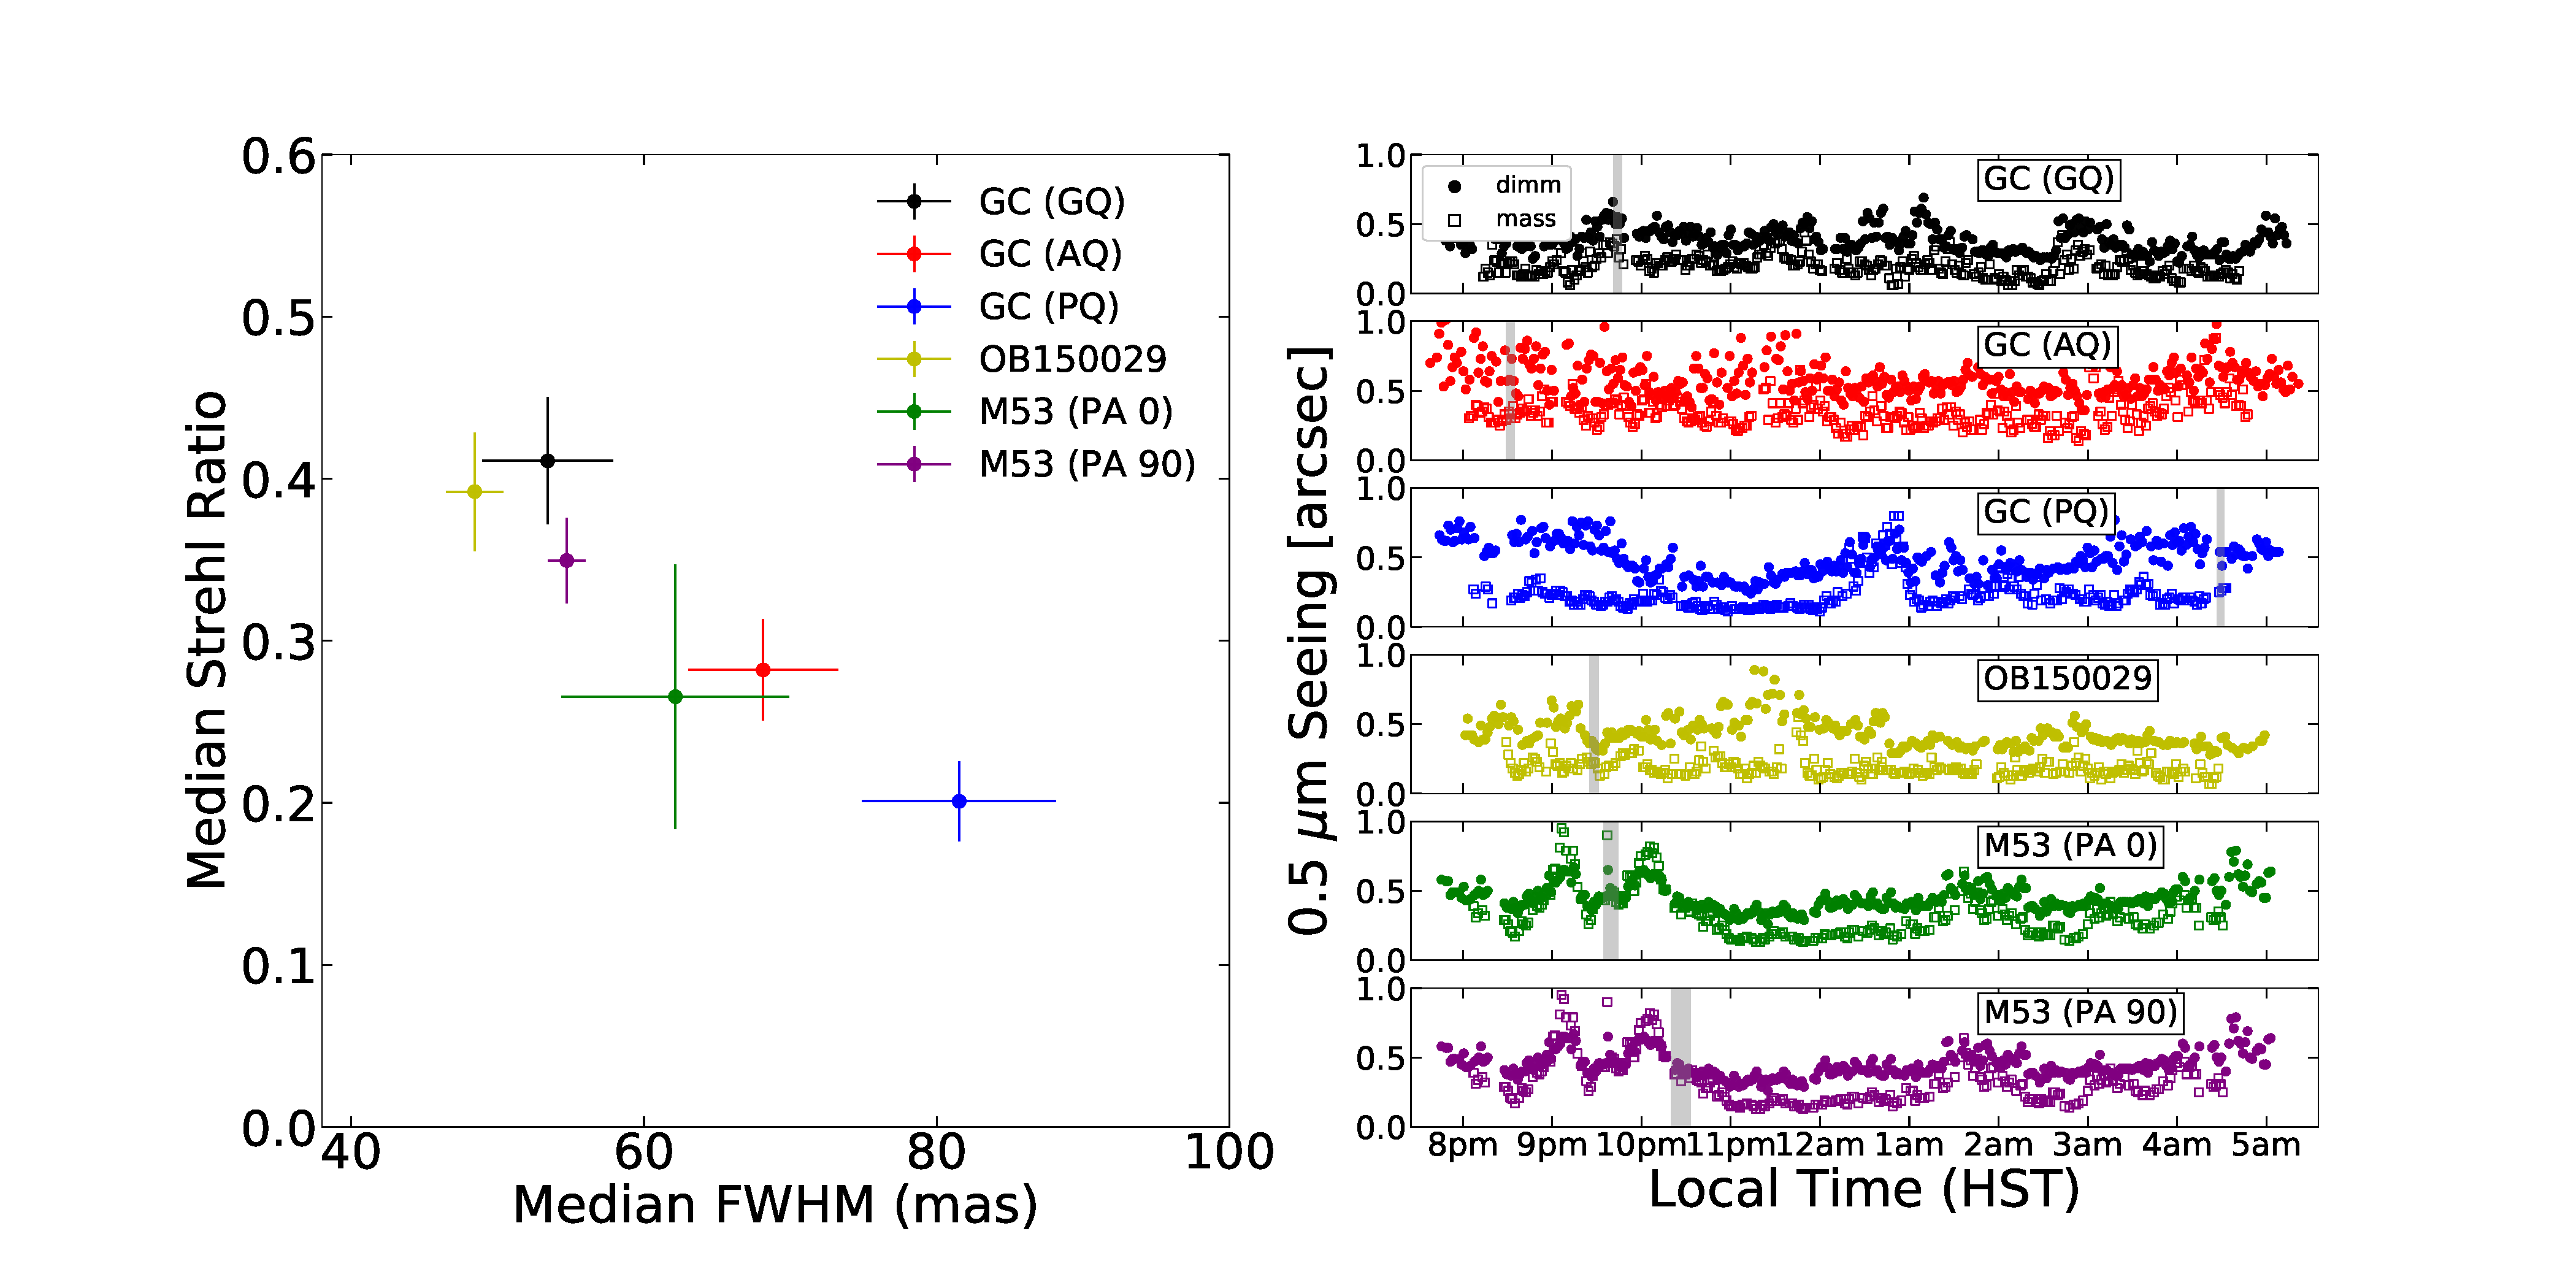
\includegraphics[width=1.2\textwidth]{Figures/metrics_dimmmass.pdf}
 }
 \caption{\footnotesize \textit{Left}: Strehl ratio and FWHM median and standard deviation for all datasets analyzed in this work. \textit{Right}: 0.5$\mu m$ DIMM/MASS seeing profiles for each dataset, respectively. Grey shaded region represents time of observation for each set. Six cleaned frames were analyzed for each dataset. \label{fig:dimmmass_datasets}}
\end{figure}

\noindent A total of six cleaned frames from each dataset were reduced identically with a NIRC2 pipeline to correct instrumental effects \citep{ghez:2008a, lu:2008a} and apply geometric distortion corrections \cite{lu:2008a, service:2016a}. North is up and East is left in all observations, with one exception for the PA $=$ 90 observations where East is up and South is left.

There are many reasons to include a wide range of variable condition data across different stellar fields on-sky, which include; testing the effects of varying DIMM/MASS profiles on PSF extraction (Section \ref{sec:gc-data}), testing the fitting precision on datasets with more/less PSF reference stars in the field (i.e. crowded/sparse fields, Sections \ref{sec:ogle-data} and \ref{sec:m53-data}), and determining the reliability of goodness-of-fit and other PSF fitting residuals for extracted sources (Sections \ref{sec:fvu} and \ref{sec:fvu-astrom-results}).

\begin{table}[!h]
\centering
\caption{Observational data presented in Sections \ref{sec:gc-data}, \ref{sec:ogle-data}, and \ref{sec:m53-data}.} \label{tab:fields-metrics}
\begin{tabular}{|l|c|c|c|c|c|}
\hline
        Field &  Date [UT] &  Strehl Ratio &  FWHM [mas] &  RMS WFE [nm] & Exp. Time [s] \\\hline\hline
        GC (GQ) &   2017 Aug 11 & $0.41 \pm 0.039$ & $53 \pm 4.5$ & $320 \pm 18$ & 168\\
        GC (AQ) &   2017 Aug 23 & $0.29 \pm 0.024$ & $66 \pm 3.5$ & $380 \pm 13$ & 168\\
        GC (PQ) &   2016 May 03 & $0.21 \pm 0.025$ & $82 \pm 6.6$ & $430 \pm 18$ & 168\\
        OB150029 &    2016 Jul 14 &  $0.39 \pm 0.037$ & $48 \pm 1.9$ & $330 \pm 17$ & 180\\
        M53 (PA$=$0) &   2015 May 05 &  $0.27 \pm 0.081$ & $62 \pm 7.8$ & $390 \pm 44$ & 300\\
        M53 (PA$=$90) &   2015 May 05 & $0.35 \pm 0.026$ & $55 \pm 1.3$ & $350 \pm 12$ & 300\\\hline
\end{tabular}
\end{table}

\subsection{Galactic Center: A Crowded Field in Varying Conditions} \label{sec:gc-data}
We expand upon the initial on-sky GC testing of \cite{Turri:inprep} by including ``good quality", ``average quality", and ``poor quality" datasets (hereafter GQ, AQ, and PQ respectively) for further AIROPA validations on the GC. The GC case was used as the main science driver for the original development of AIROPA. This case is ideal since there already exists a rich high-resolution dataset spanning several decades, dozens of reference stars for PSF modeling, and a very bright, uniform tip/tilt (TT) guide star that is ${\sim}13$ arcseconds off-axis. The longest-running high-resolution study of the stellar population immediately surrounding Sgr A$^{*}$ is being conducted by the Galactic Center Orbit Initiative \textbf{(footnote to GCG webpage or something?)}. This work has led to a deep and well-understood knowledge \citep{ghez:2005b, ghez:2008a, lu:2008a, do:2019a, gautam:2019a} of the environment immediately surrounding the central supermassive black hole.

\begin{figure}[!h]
 \makebox[\textwidth][c]{
 \hspace*{-0.5cm}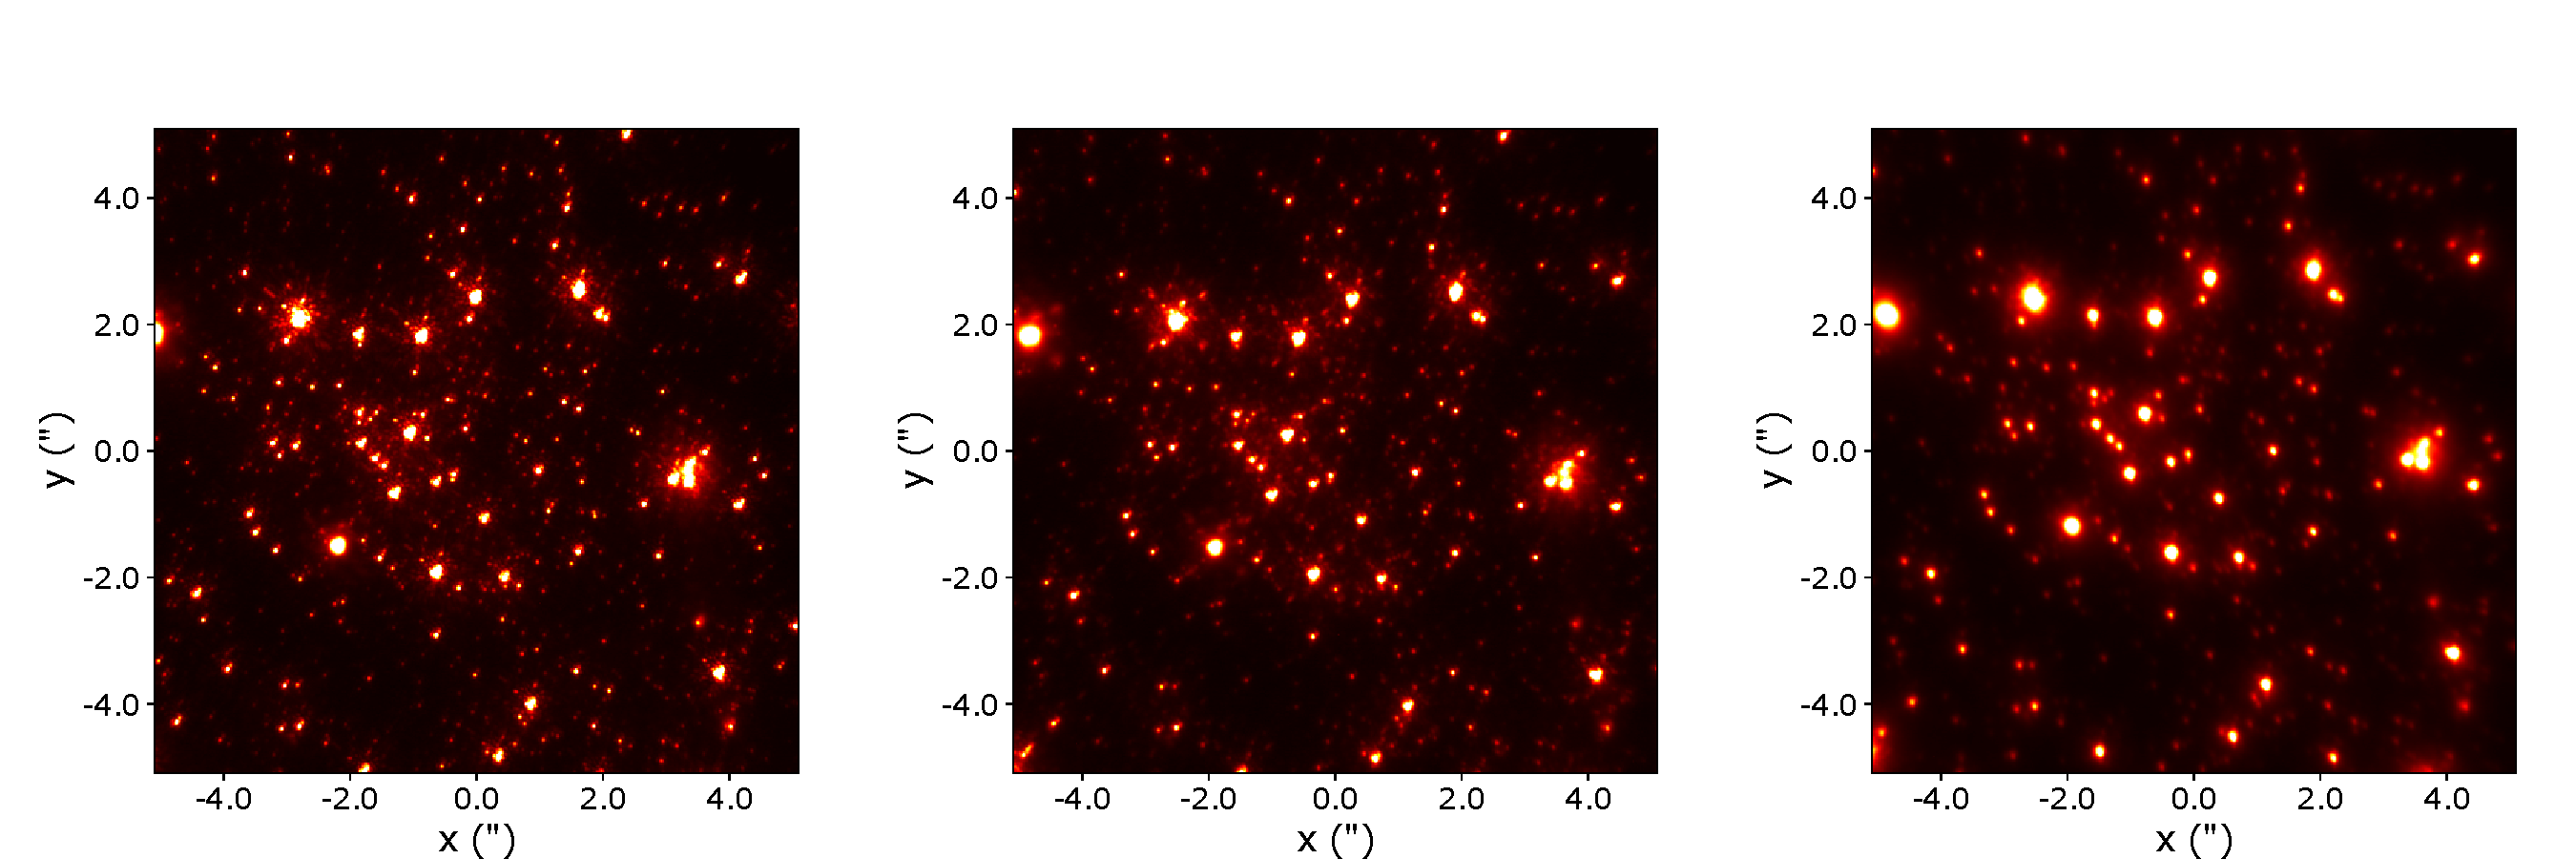
\includegraphics[width=1.15\textwidth]{Figures/gc_images.pdf}
 }
 \caption{\footnotesize \textit{Left}: Good-quality Galactic Center frame. \textit{Middle}: Average-quality Galactic Center frame. \textit{Right}: Poor-quality Galactic Center frame. All images have the same color scale, the axes represent on-sky separation (in arcsec) from the on-axis (i.e. center) frame position. \label{fig:gc_images}}
\end{figure}

\begin{figure}
 \makebox[\textwidth][c]{
 \hspace*{0.5cm}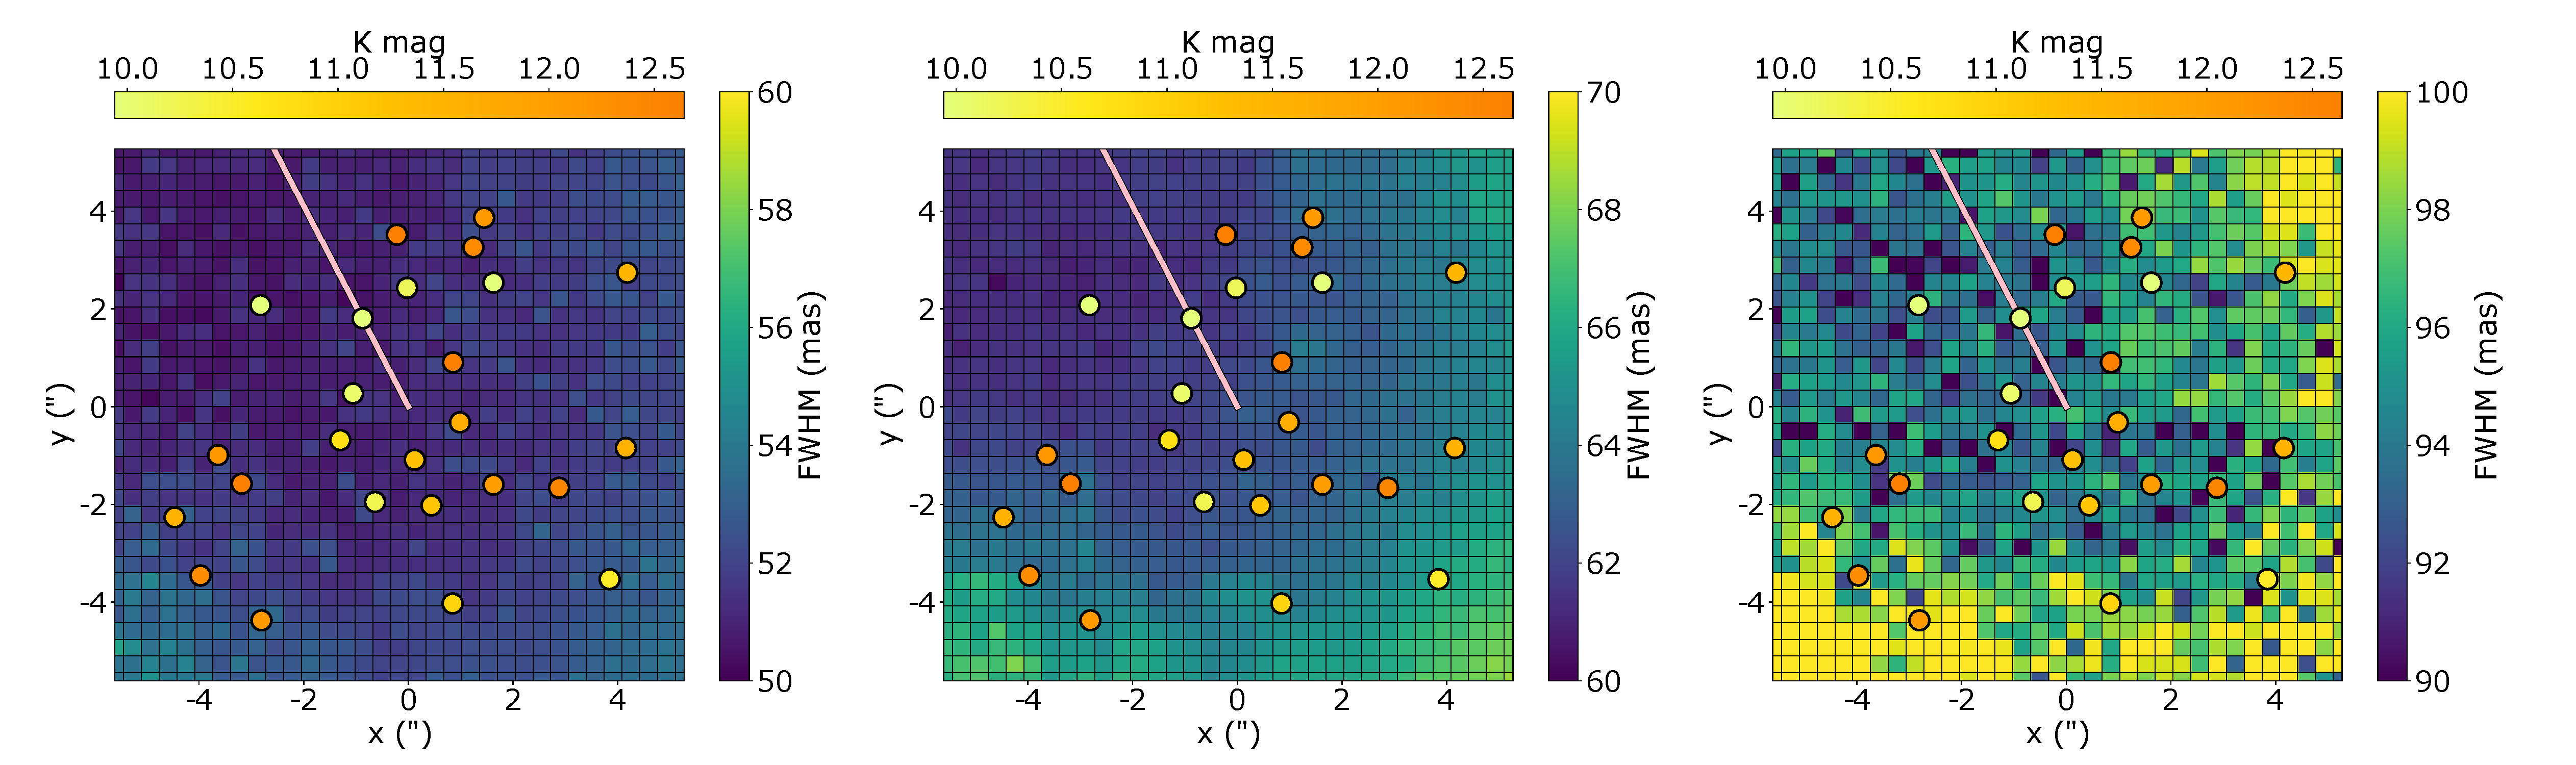
\includegraphics[width=1.2\textwidth]{Figures/fwhm_grids.pdf}
 }
 \caption{\footnotesize Grid of FWHM values from AIROPA variable-PSF mode on the GQ (\textit{left}), AQ (\textit{middle}) and PQ (\textit{right}) datasets. Colored circle points correspond to locations and K-band magnitudes of primary PSF reference stars. A straight line connects the on-aixs LGS position to the off-axis TT guide star position. \label{fig:fwhm_grids}}
\end{figure}

\indent We rank the three GC datasets, GQ, AQ, and PQ based on the historical quality of all GC epochs taken with NIRC2 since 2004 \citep{jia:2019a}. Figure \ref{fig:dimmmass_datasets} shows the median Strehl and FWHM values and standard deviations for all datasets analyzed in this work. The GQ, AQ, and PQ datasets correspond to the black, red, and blue data respectively. The right panel of Figure \ref{fig:dimmmass_datasets} shows the atmosphere profile information from the DIMM/MASS instruments for each dataset, with grey shaded regions representing the time of observation considered in this analysis. The observation timestamps span 8:30pm to 4:30am local HST time. Table \ref{tab:fields-metrics} shows the quality metrics (i.e. median strehl/FWHM/RMS WFE), observation dates, and total exposure times for all datasets analyzed.

The GQ dataset was taken on 2017-08-11, The AQ data were taken $\sim$two weeks after the GQ data, on 2017-08-23, and the PQ data were taken on 2016-05-03. Dates are given in Hawaiian standard time (HST). For all GC datasets, each frame was composed of 10 coadded exposures at 2.8s per coadd for a total exposure time of 28s per frame. One note about the PQ dataset; there does not exist phase diversity calibration data from 2016, therefore the 2017 instrumental phase maps were used to substitute for the 2016 phase maps. This is not an issue, as \cite{Ciurlo:inprep} show that the phase maps can remain stable across multiple years, and any potential difference between 2016 and 2017 phase diversity is likely small enough for an analysis of the kind presented in this work. Figure \ref{fig:gc_images} shows one frame from each of the three epochs, with the spatial scale given as the separation (in arcseconds) from the on-axis position (i.e. image center). Figure \ref{fig:fwhm_grids} shows the grid of FWHM values measured by AIROPA variable-PSF mode for each frame, plotted over the field of view to give a visualization of the field-dependent PSF. The FWHM grid values are calculated for every PSF generated by AIROPA in the PSF grid file, \textit{*\_on\_axis\_psf.fits}. The AIROPA grid files for the fields analyzed in this work use a partition size (i.e. step width of the PSF grid) of 102. 

%Regarding FVU on bright/faint stars.

%\begin{figure}
% \makebox[\textwidth][c]{
% 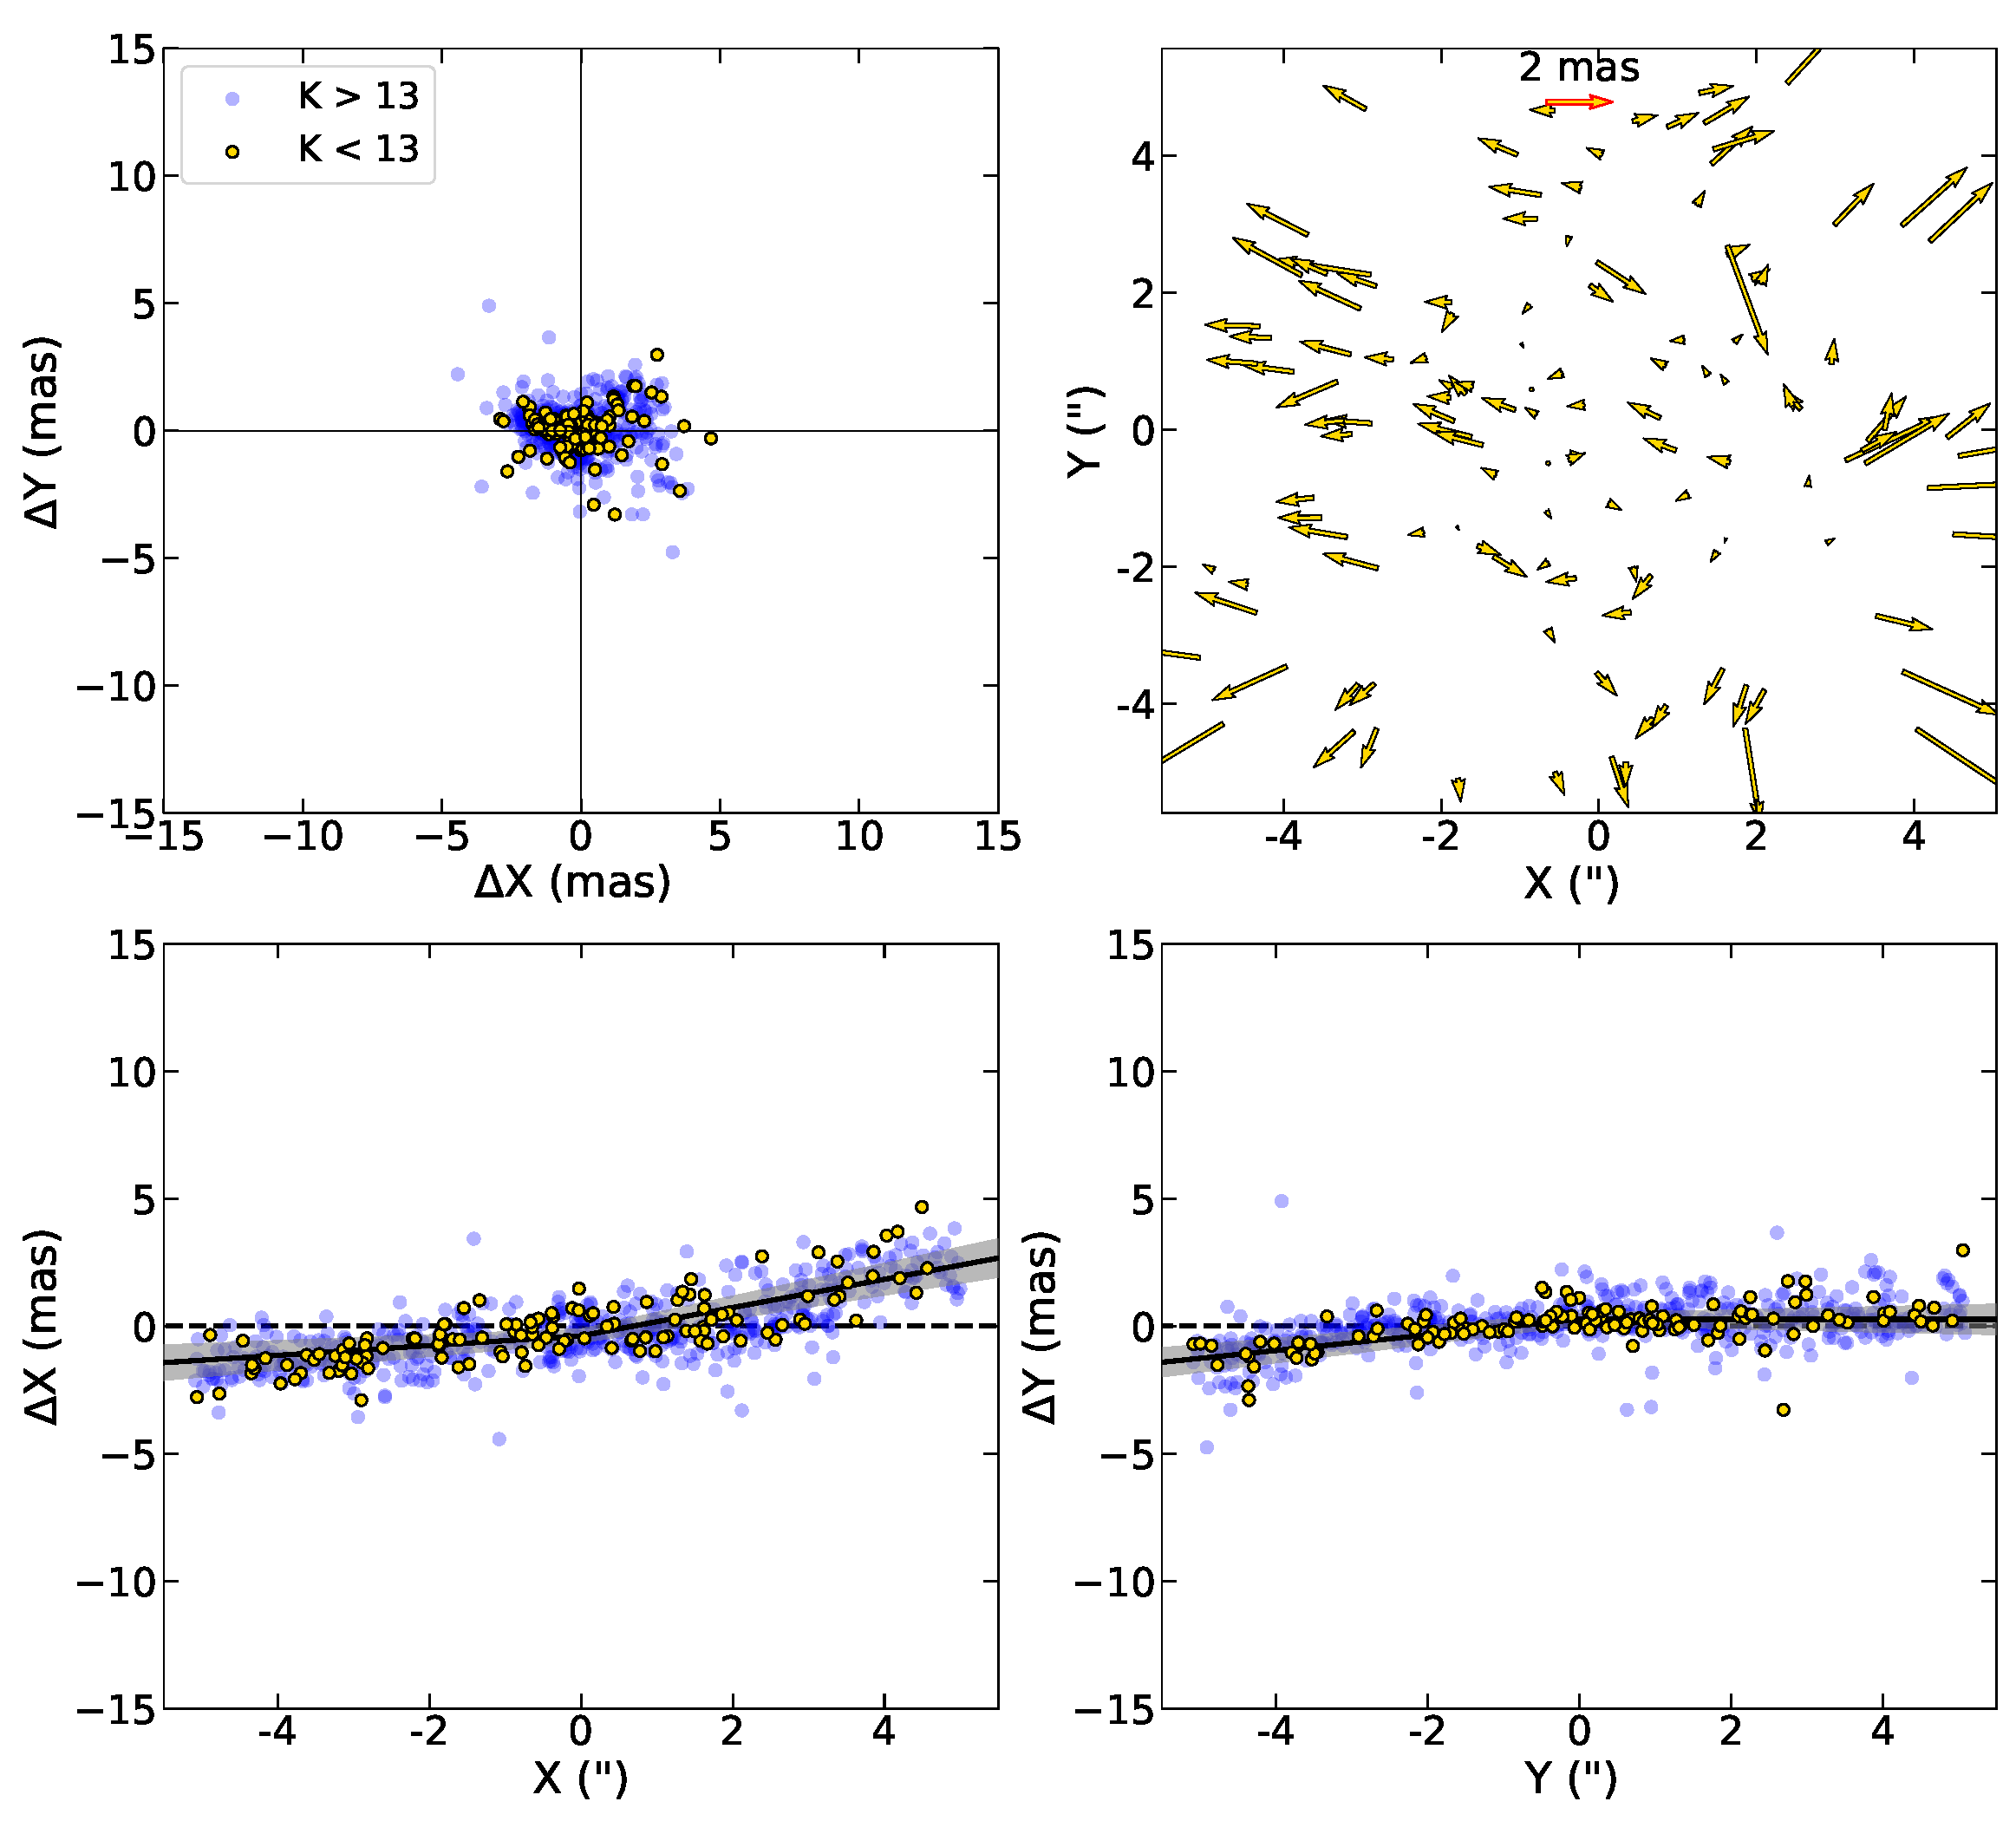
\includegraphics[width=1.0\textwidth]{Figures/SV_astrometry_quad.pdf}
% }
% \caption{\footnotesize \textit{Top-left}: Averaged positional difference in X and Y between single and variable-PSF modes for the AQ dataset. Yellow data corresponds to K $<$ 13 stars, blue data shows all stars detected. \textit{Top-right}: Quiver plot showing the astrometric differences. \textit{Lower-left}: Astrometric difference as a function distance from the central pointing in X directions. \textit{Lower-right}: Same as lower-left, but for Y directions. The solid black line shows a third-order polynomial fit to all data points, with a shaded region representing 1$\sigma$ spread about the mean. \label{fig:gc_astrom}}
%\end{figure}

%----------------AIROPA ON OB150029------------------------------------------------------------------------------------------------------------
 
\subsection{OGLE-2015-BLG-0029: A Less Crowded Microlensing Field} \label{sec:ogle-data}
The Optical Gravitational Lensing Experiment (OGLE) survey \cite{udalski:1992a} conducts wide-field visible and near-IR imaging of nearly the entire Galactic Bulge region at high cadence, and detects over 1000 microlensing events every season. Most ground-based imaging data from current microlensing surveys are focused in regions $3\degree > l > 357\degree$ and $-2.5\degree < b < 2.5\degree$. The first non-GC data analyzed in this work is OGLE-2015-BLG-0029 (hereafter OB150029), located at RA $=$ 17:59:46.60, DEC $=$ -28:38:41.80 and Galactic coordinates ($l,b = (1.828\degree, -2.523\degree$)). This target has been regularly monitored with NIRC2 since 2015 as part of a project to study isolated stellar-mass black hole candidates \citep{lu:inprep}.

\begin{figure}[!h]
 \makebox[\textwidth][c]{
 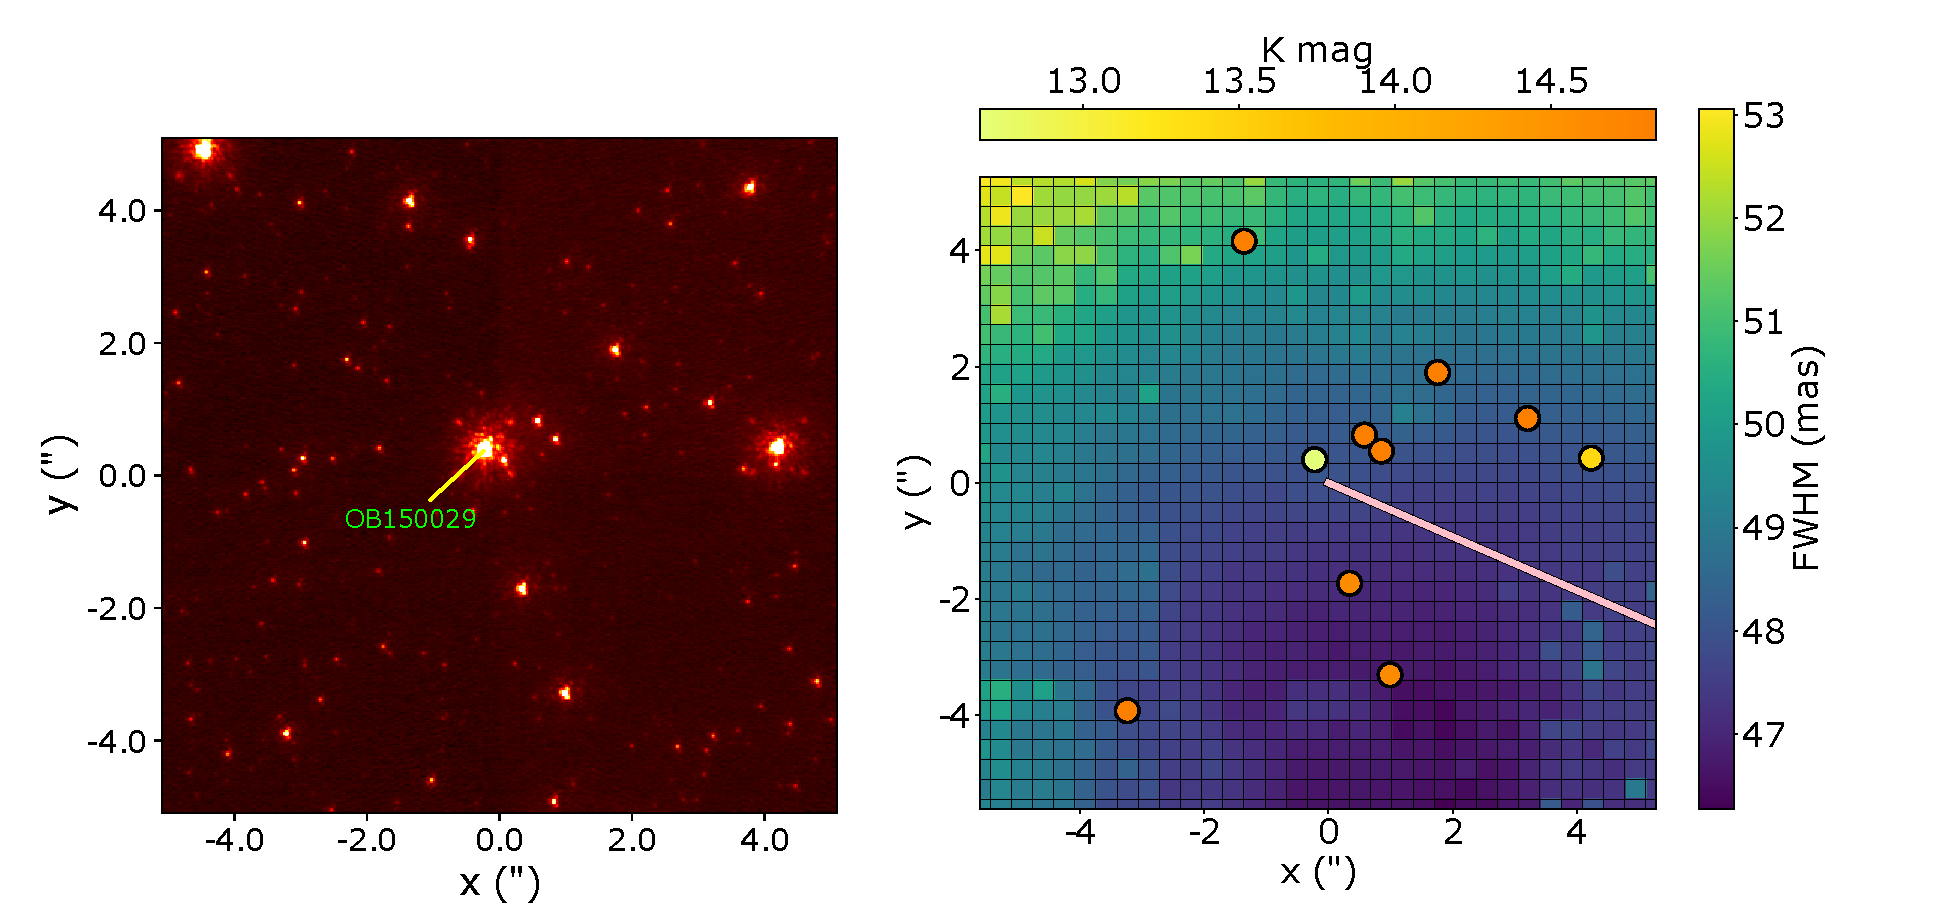
\includegraphics[width=1.1\textwidth]{Figures/nirc2-ob150029.pdf}
 }
 \caption{\footnotesize \textit{Left}: NIRC2 frame of the OB150029 field taken on 2016-07-14 with the Kp filter. \textit{Right}: FWHM grid from AIROPA variable-PSF mode with selected PSF reference stars colored by magnitude and solid line connecting the on-axis position to the TT star.} \label{fig:ob150029}
\end{figure}

The OB150029 observations were taken on 2016-07-14 in LGSAO mode with the Kp filter. Each of the frames consist of six co-added images, each with five second integration time, for a total integration time of 30 seconds per frame. The airmass during the six-frame observing window was $\sim$1.65, and the median Strehl, FWHM, and RMS WFE values for the six frames are given in Table \ref{tab:fields-metrics}, as well as the DIMM/MASS data given on the right-hand panel of Figure \ref{fig:dimmmass_datasets}. This is the second-best dataset (behind GQ) in terms of quality metrics like the median Strehl and FWHM and their variances across all six frames. Similar to the PQ dataset, there are no 2016 phase maps available for NIRC2, therefore the 2017 maps were substituted. Again, phase diversity measurements have shown these maps to be relatively stable across several years \citep{Ciurlo:inprep}. Figure \ref{fig:ob150029} shows a NIRC2 image of the field, which is clearly less crowded than the GC. 

\indent There are a total of 10 PSF reference stars in this field that were used for AIROPA, compared to a total of 25 PSF reference stars used for the GC analysis described in Section \ref{sec:gc-data}. The total number and spatial location of selected PSF reference stars is important for constructing accurate PSF models, and the 10 stars chosen for the OB150029 field include the target itself, stars with $m_K = \pm 1.5$ mag of the target and separation of $\pm4.0$ arcseconds from the target. The TT guide star used for the observations has an R mag ${\sim}$15.1 and separation of ${\sim}$13.8 arcseconds to the Southwest of the target, as indicated by the solid line in the right panel of Figure \ref{fig:ob150029}.

\begin{figure}[!h]
 \makebox[\textwidth][c]{
 \hspace*{-0.5cm}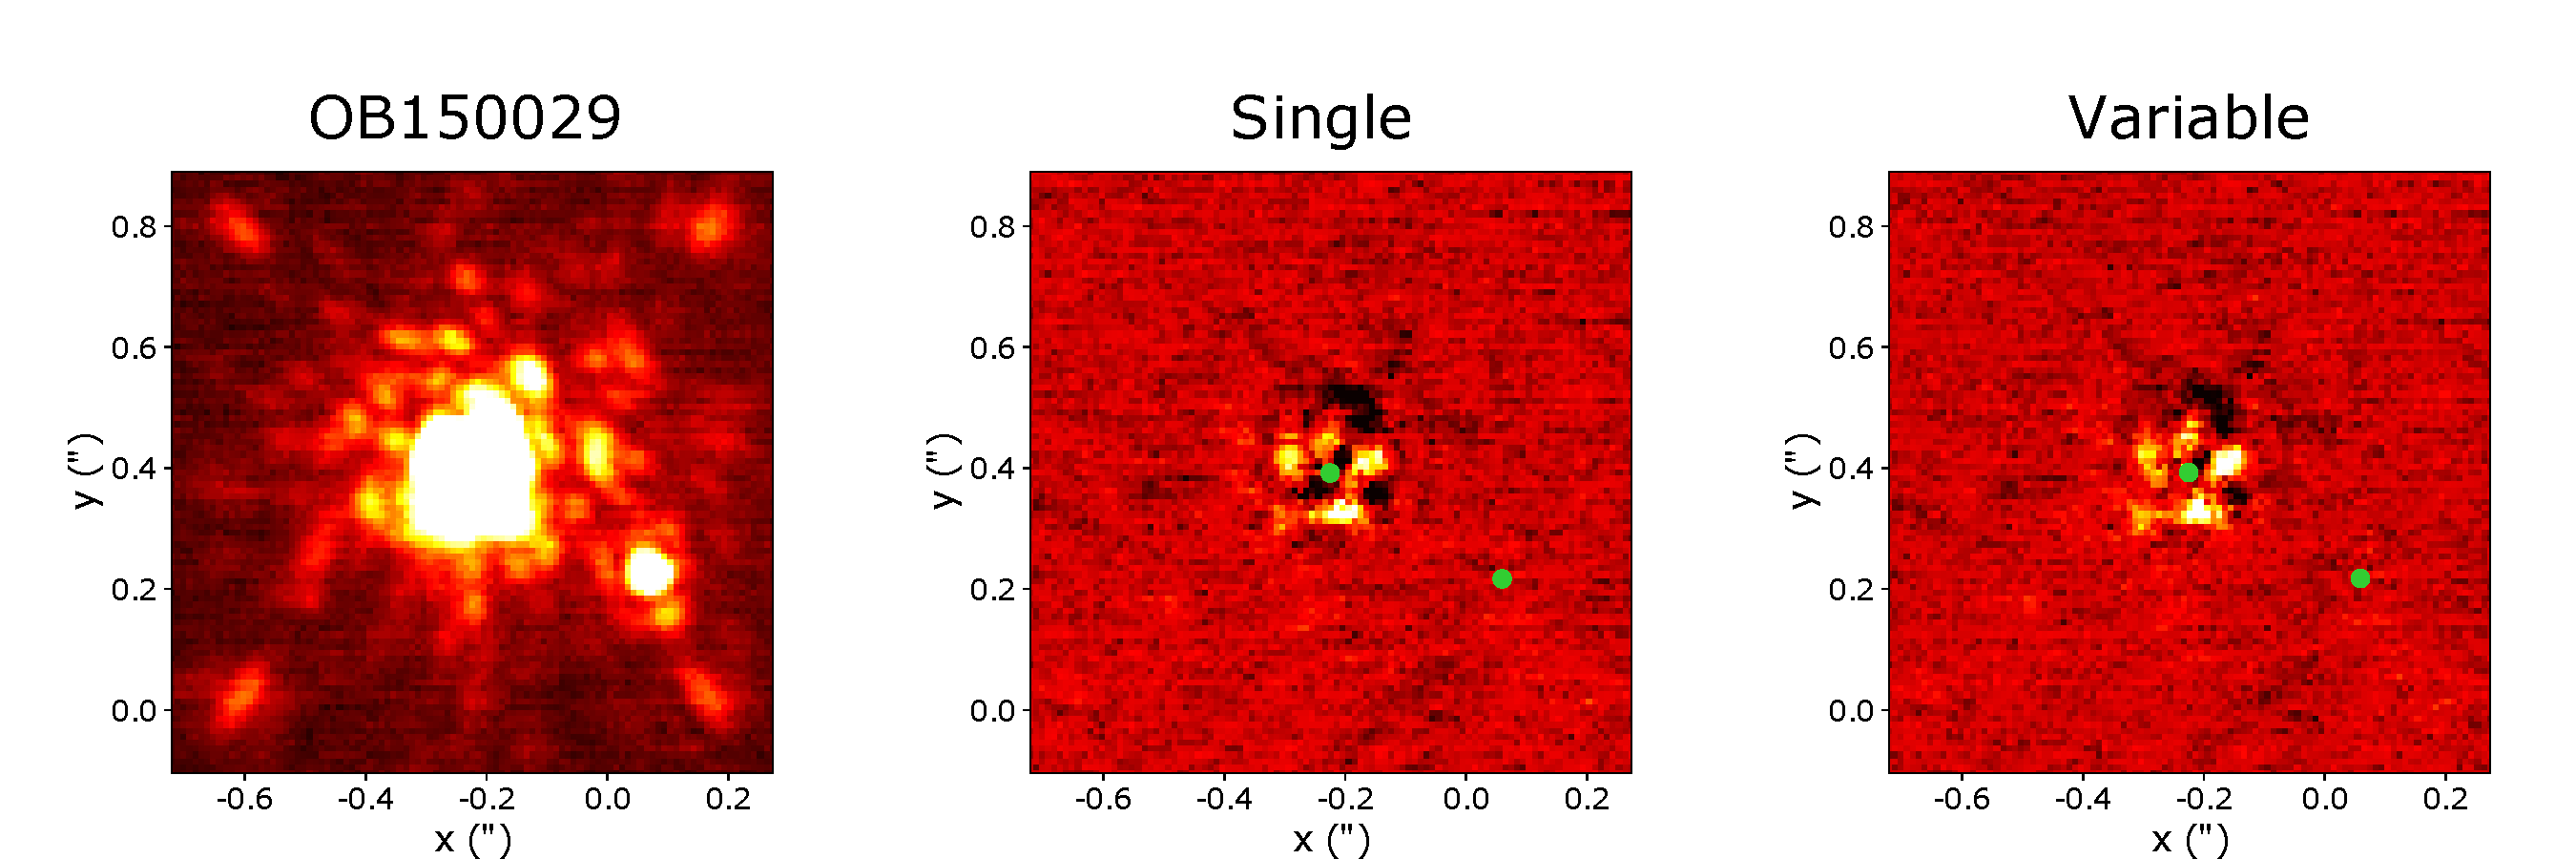
\includegraphics[width=1.1\textwidth]{Figures/ob150029_targ_res.pdf}
 }
 \caption{\footnotesize Single image of the target OB150029 (\textit{left}) and residual images from the single-PSF (\textit{middle}) and variable-PSF (\textit{right}) modes. Residual images have identical color scales, and green points show the location of star detections.} \label{fig:ob150029-targ-res}
\end{figure}

%----------------AIROPA ON M53------------------------------------------------------------------------------------------------------------

\subsection{M53: A Globular Cluster at Different Position Angles} \label{sec:m53-data}
The globular cluster M53 (NGC 5024) located at RA $=$ 13:12:54.51, DEC $=$ 18:10:13.95 was observed with the NIRC2 narrow camera Kp filter on 2015-05-04 as part of a project to characterize the NIRC2 geometric distortion \cite{service:2016a}. This was accomplished by comparing the NIRC2 stellar positions to precise astrometry from \textit{Hubble Space Telescope} (HST) \textit{Advanced Camera for Surveys} (ACS) observations. The NIRC2 camera and AO system was realigned in April 2015, and observations of M53 before and after this realignment show an increase in the averaged geometric distortion from $\sim$0.5 mas pre-realignment to $\sim$1.1 mas post-realignment.

\begin{figure}[!htb]
 \makebox[\textwidth][c]{
 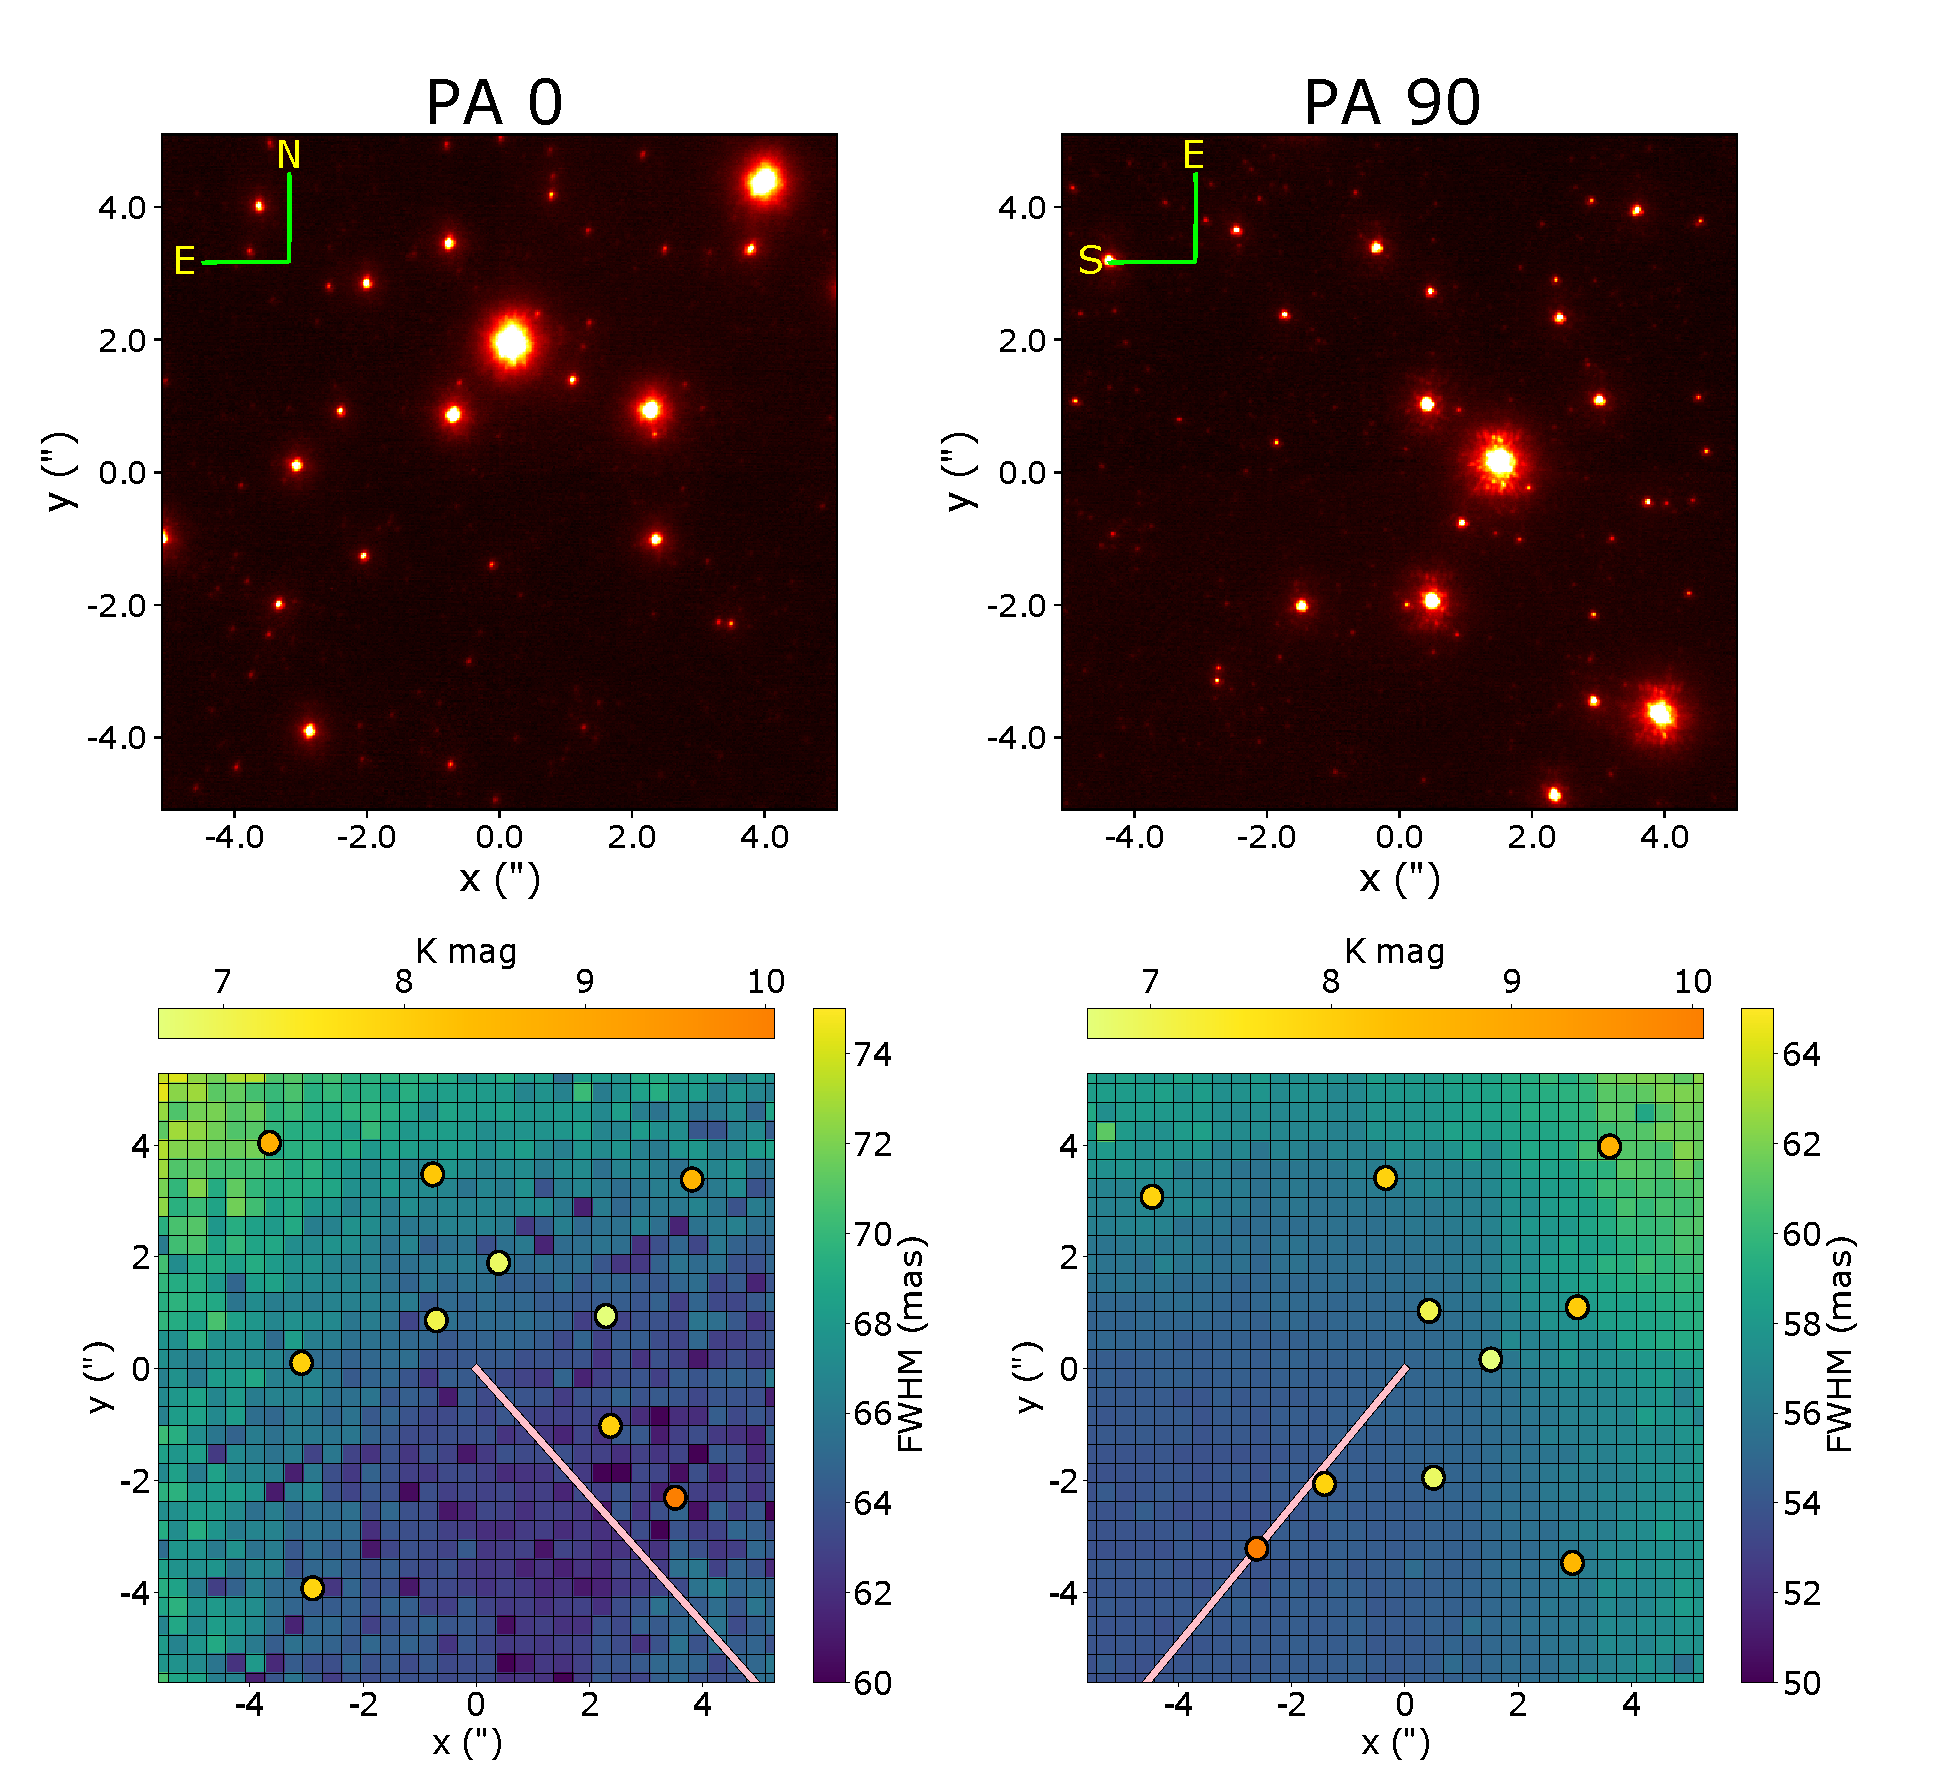
\includegraphics[width=1.0\textwidth]{Figures/quad-m53.pdf}
 }
 \caption{\footnotesize \textit{Left Column}: M53 NIRC2 frame taken at PA = 0, with accompanying FWHM grid generated by AIROPA. \textit{Right Column}: Same as left, but for PA = 90.} \label{fig:m53_image_grid}
\end{figure}

Importantly, the NIRC2 observations were taken at two different position angles (PA); 0$\degree$ and 90$\degree$. These prior observations present a unique dataset for us to compare the astrometric accuracy between single-PSF and variable-PSF modes in AIROPA as a function of PA. As shown in \cite{Turri:inprep}, the astrometric differences between single-PSF mode and variable-PSF mode become more severe at larger radii from the central on-axis position. This is predominantly caused by the difference in PSF shape between the spatially varying model and the static model, particularly closer to the sides and edges of the NIRC2 frame. However there is evidence that residual instrumental aberrations still persist in the system \citep{Turri:inprep}. A comparison of these astrometric differences at two different PA's may help give further insight on possible causes of the remaining aberration. Recently, it has also been shown that a dominant source of error in the PSF comes from primary segment misalignments (O. Beltramo-Martin in private communication). The work shows several hundred nm of wavefront error (WFE) coming from the primary piston segments, which can become misaligned as quickly as hours after initial alignment. Currently, the Keck-II primary mirror segments are realigned every two-weeks, however these results show that the cadence may need to be increased in order to minimize any contribution to the PSF error from this primary segment phasing.

\begin{figure}[!h]
  \centering
  \subfloat{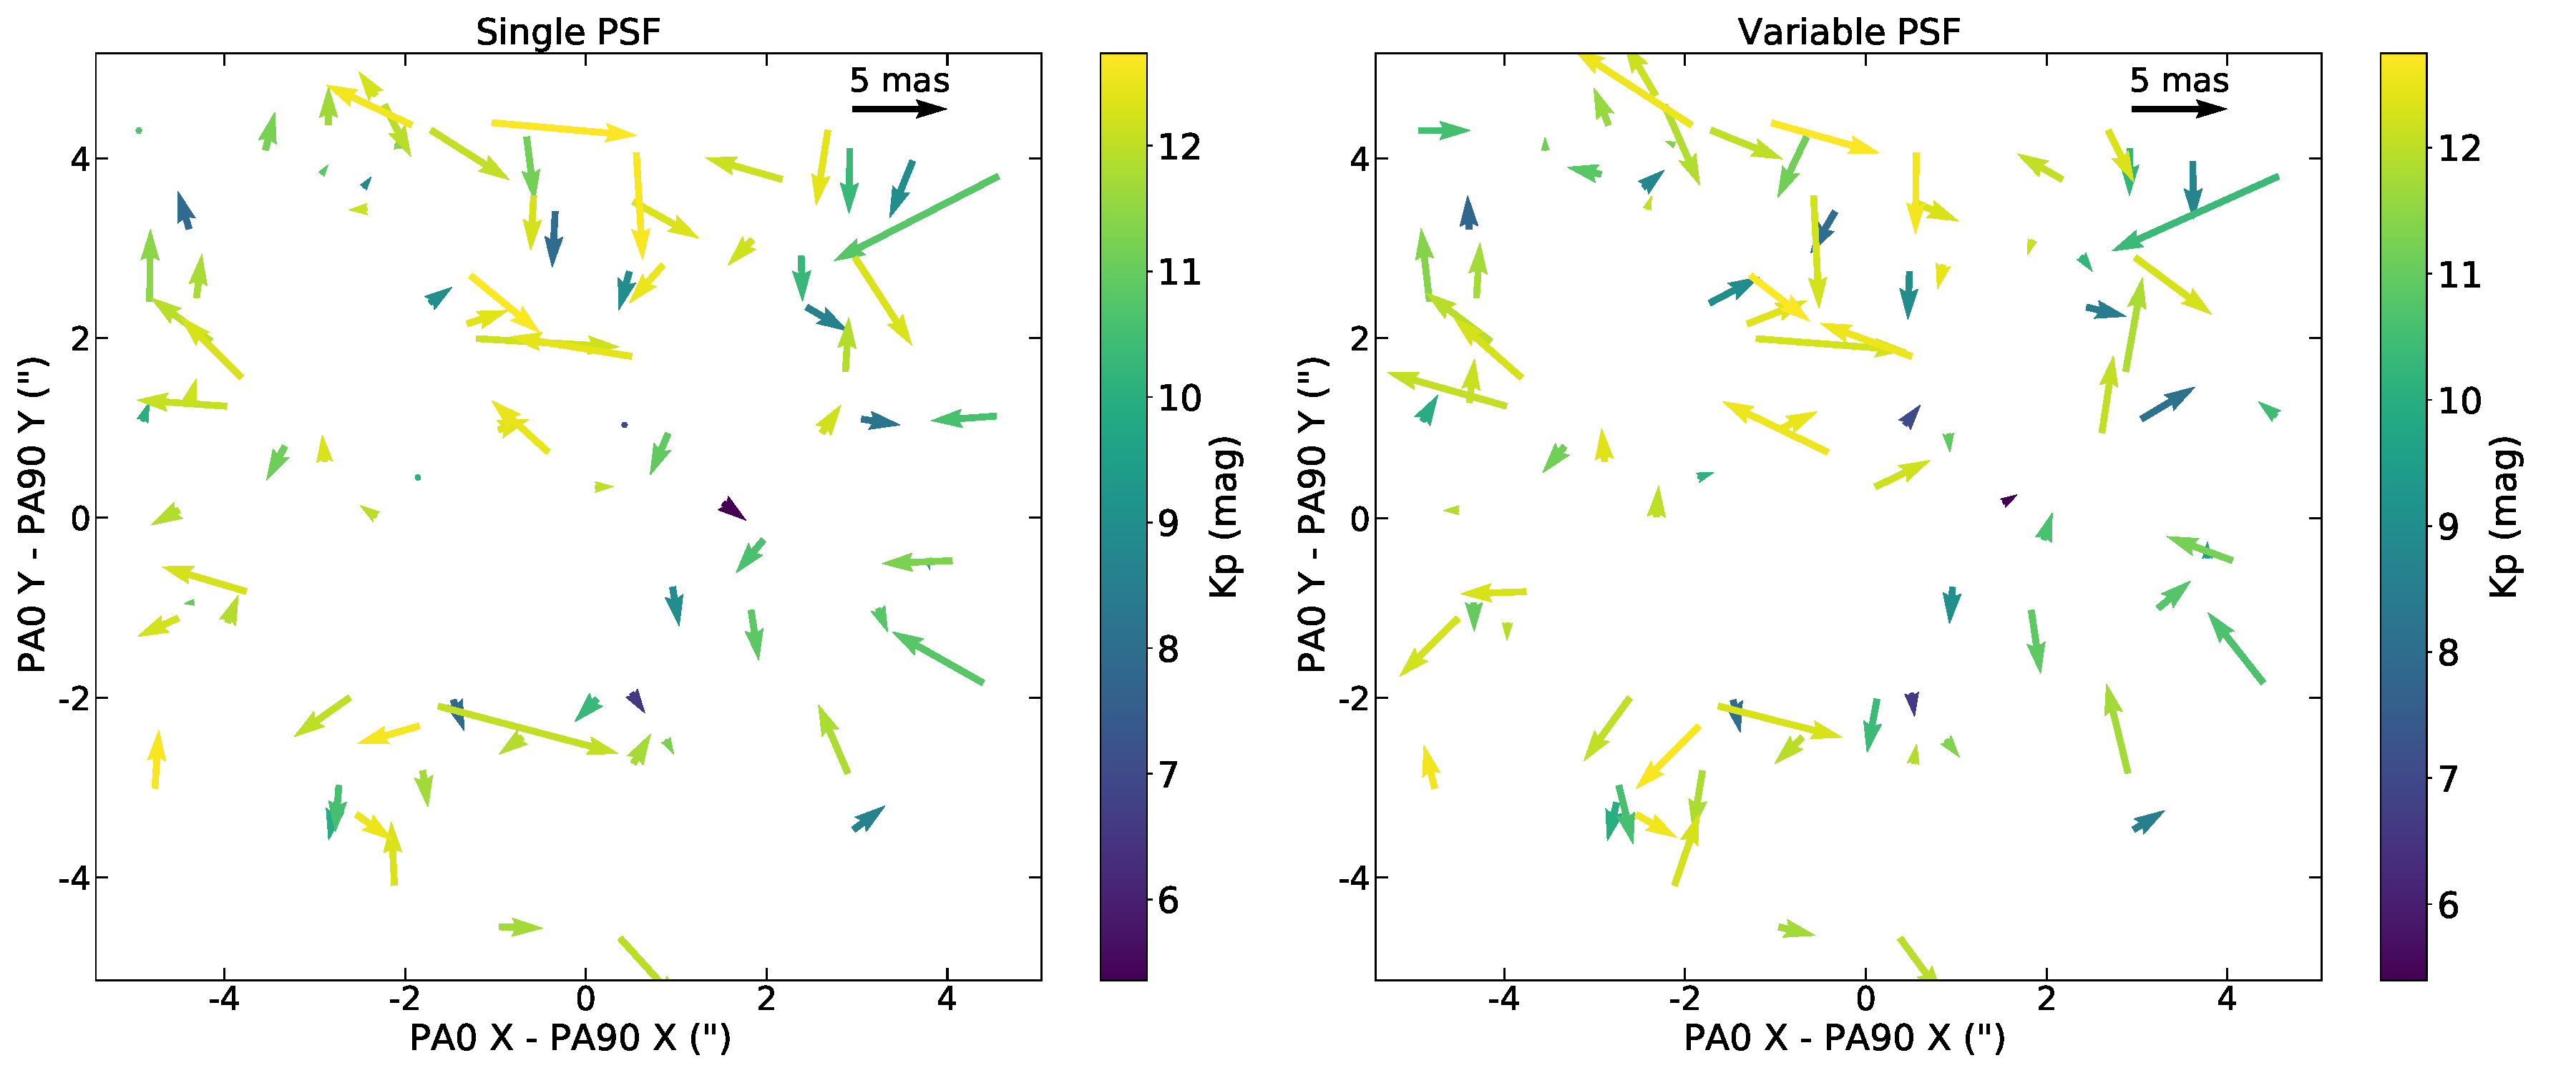
\includegraphics[width=0.95\textwidth]{Figures/m53-to-m53_both_matched_quivers.pdf}}\\
  \hspace{-1cm}
  \subfloat{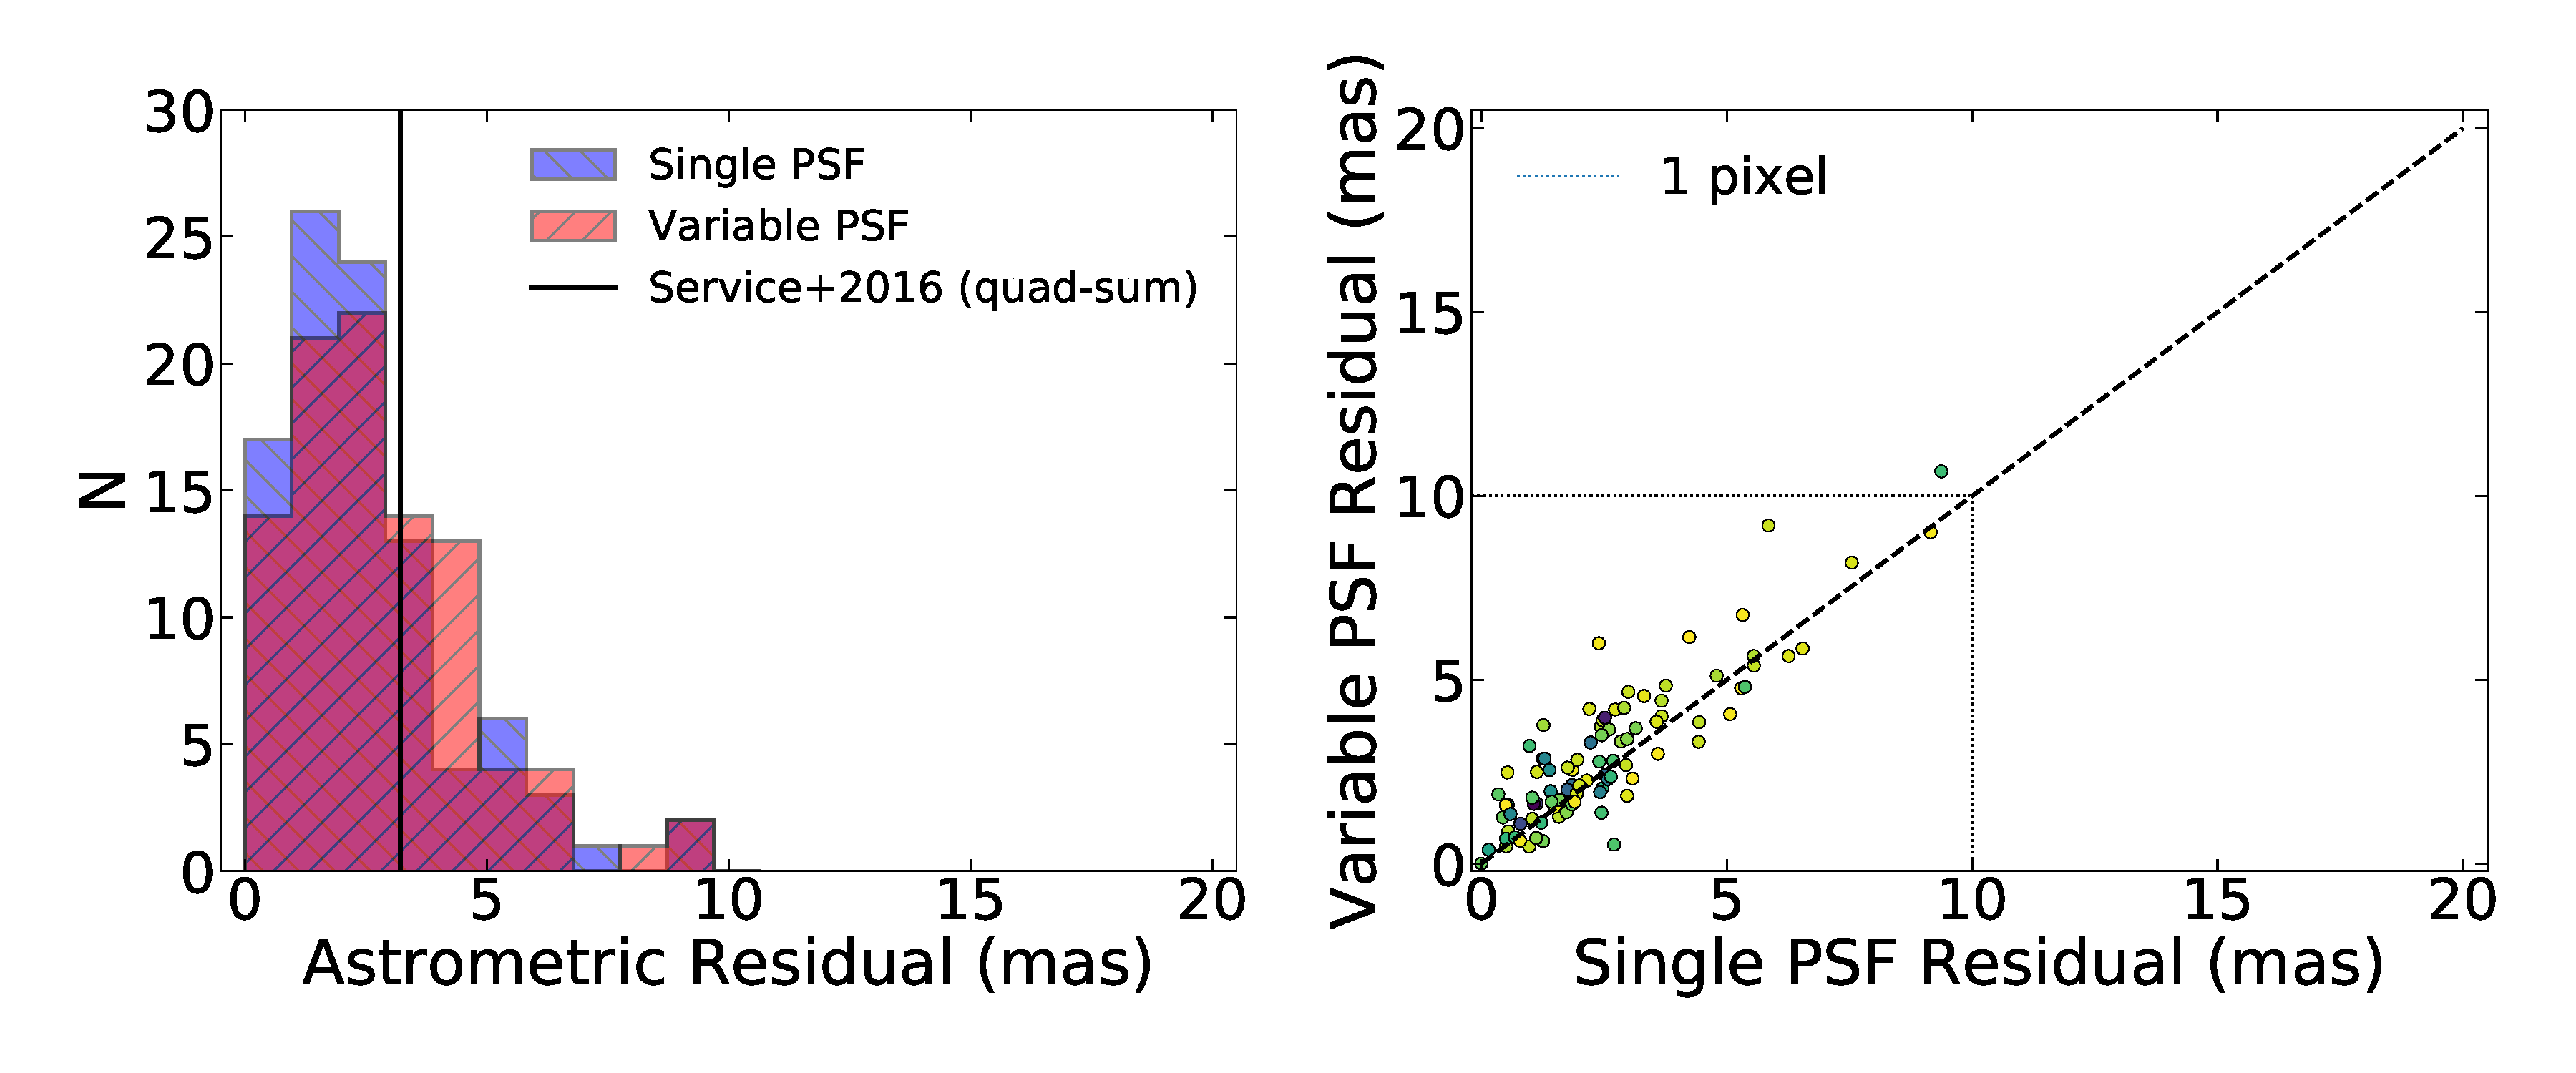
\includegraphics[width=0.95\textwidth]{Figures/m53-to-m53_histAndCorrelation.pdf}}
  \caption{\textit{Upper-left}: Quiver plot showing single-PSF astrometric residuals from the PA$=$0 $\rightarrow$ PA$=$90 transformation. \textit{Upper-right}: Same as upper-left, but for variable-PSF mode. \textit{lower-left}: Distribution of astrometric residuals from both PSF mode transformations. \textit{lower-right}: Correlation between astrometric residuals for both PSF modes.} \label{fig:m53_PA_compare}
\end{figure}

\begin{figure}[!h]
  \centering
  \subfloat{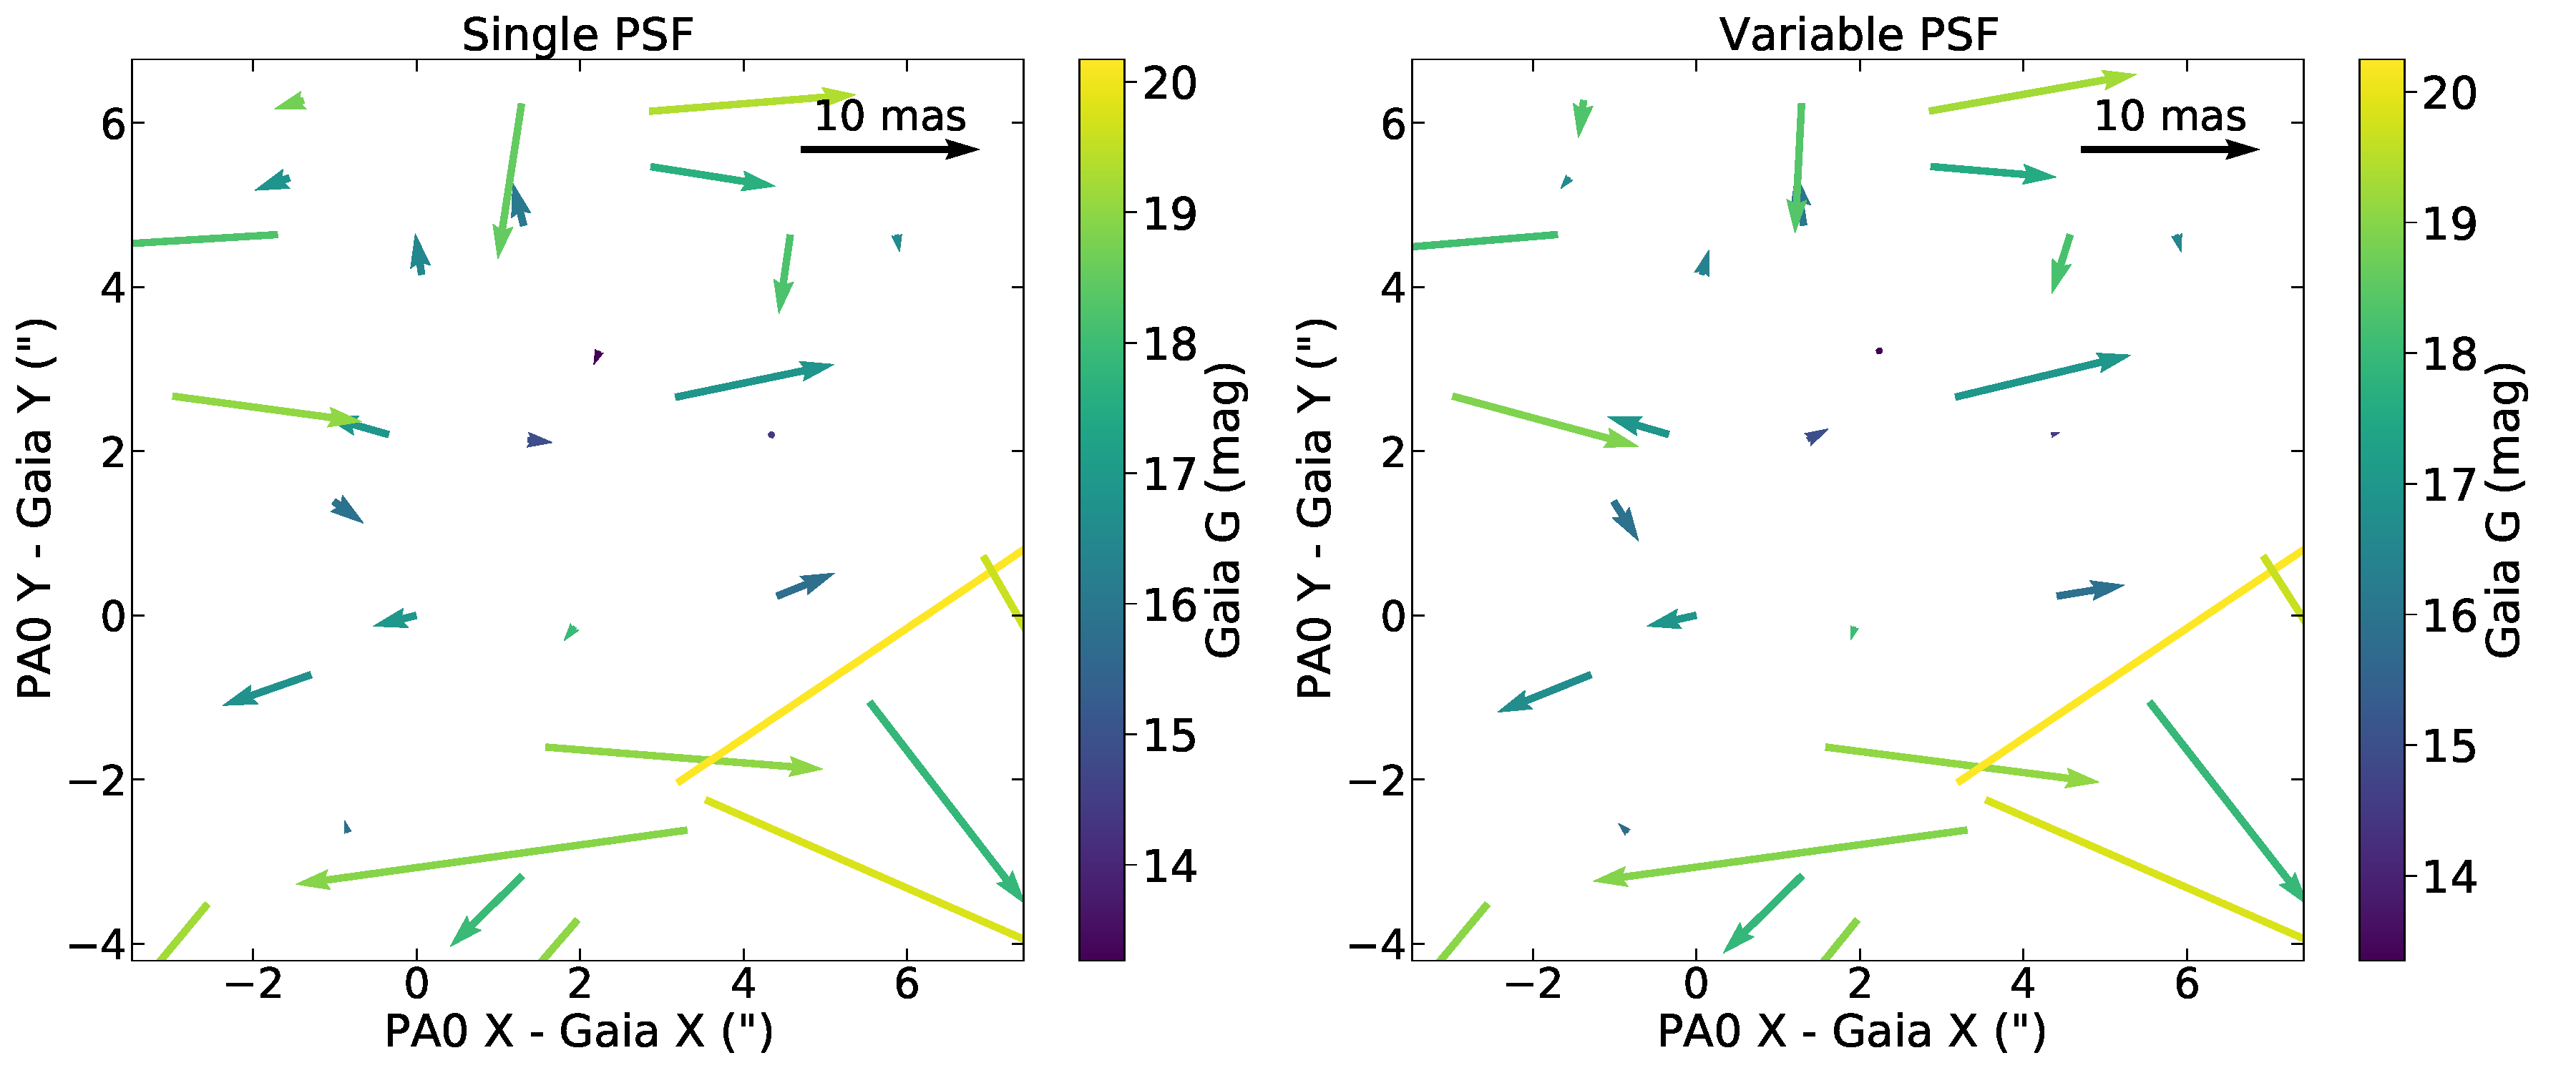
\includegraphics[width=0.95\textwidth]{Figures/m53-to-gaia_both_matched_quivers.pdf}}\\
  \hspace{-1cm}
  \subfloat{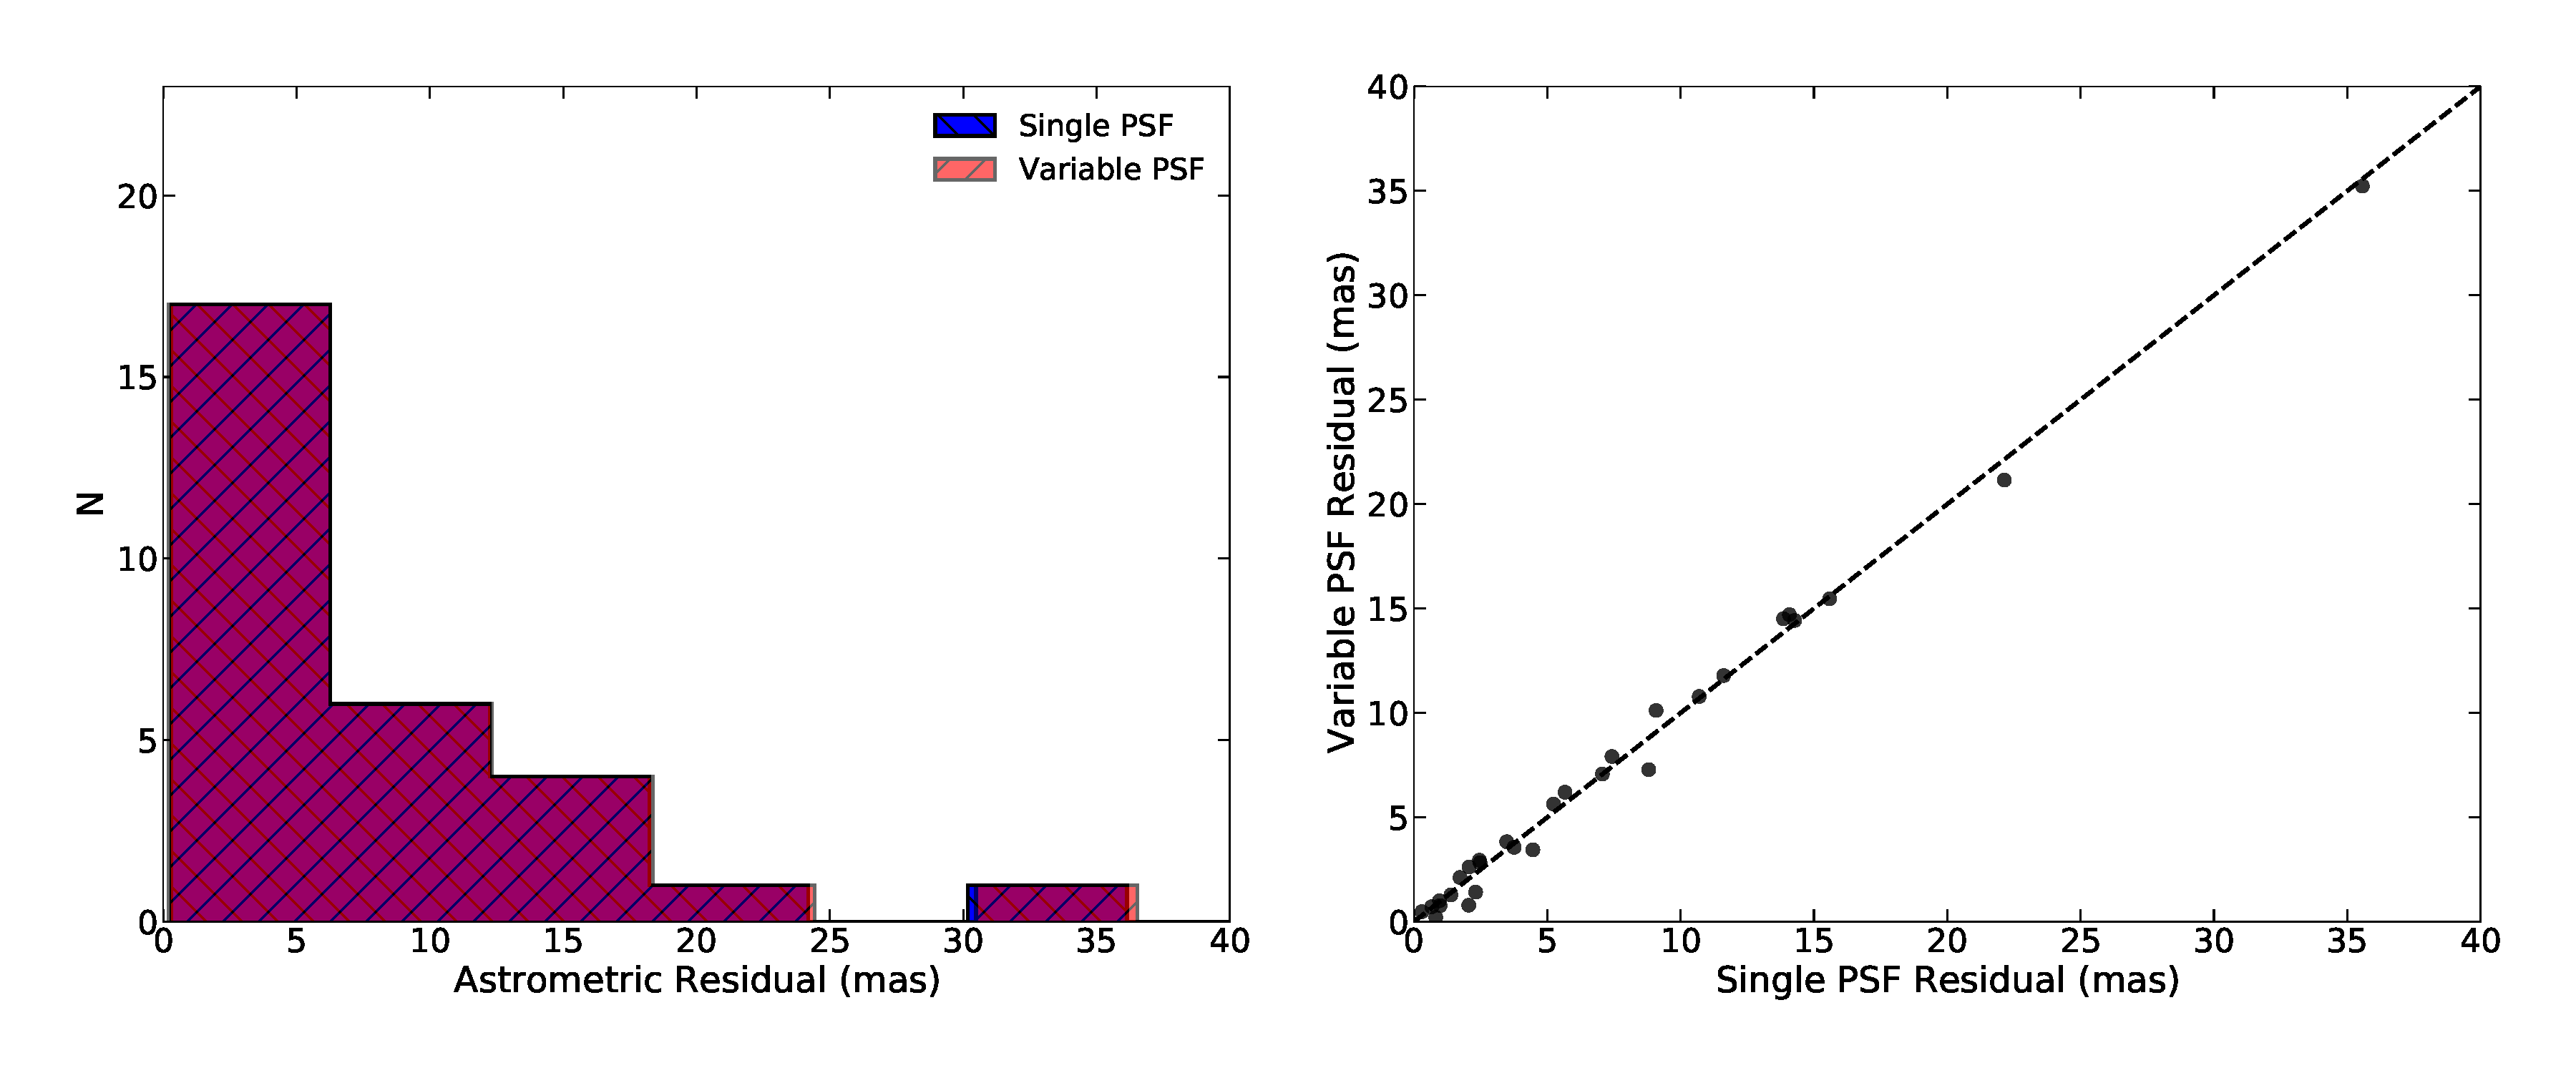
\includegraphics[width=0.95\textwidth]{Figures/m53-to-gaia_histAndCorrelation.pdf}}
  \caption{\textit{Top row}: Quiver plots similar to those in Figure \ref{fig:m53_PA_compare}, but for stars matched and transformed to Gaia EDR3. The color bar is given in Gaia G magnitude. \textit{Bottom row}: Astrometric residuals distribution and correlation between the two PSF modes.} \label{fig:m53_PA_compare_gaia}
\end{figure}

\begin{figure}[!h]
  \centering
  \subfloat{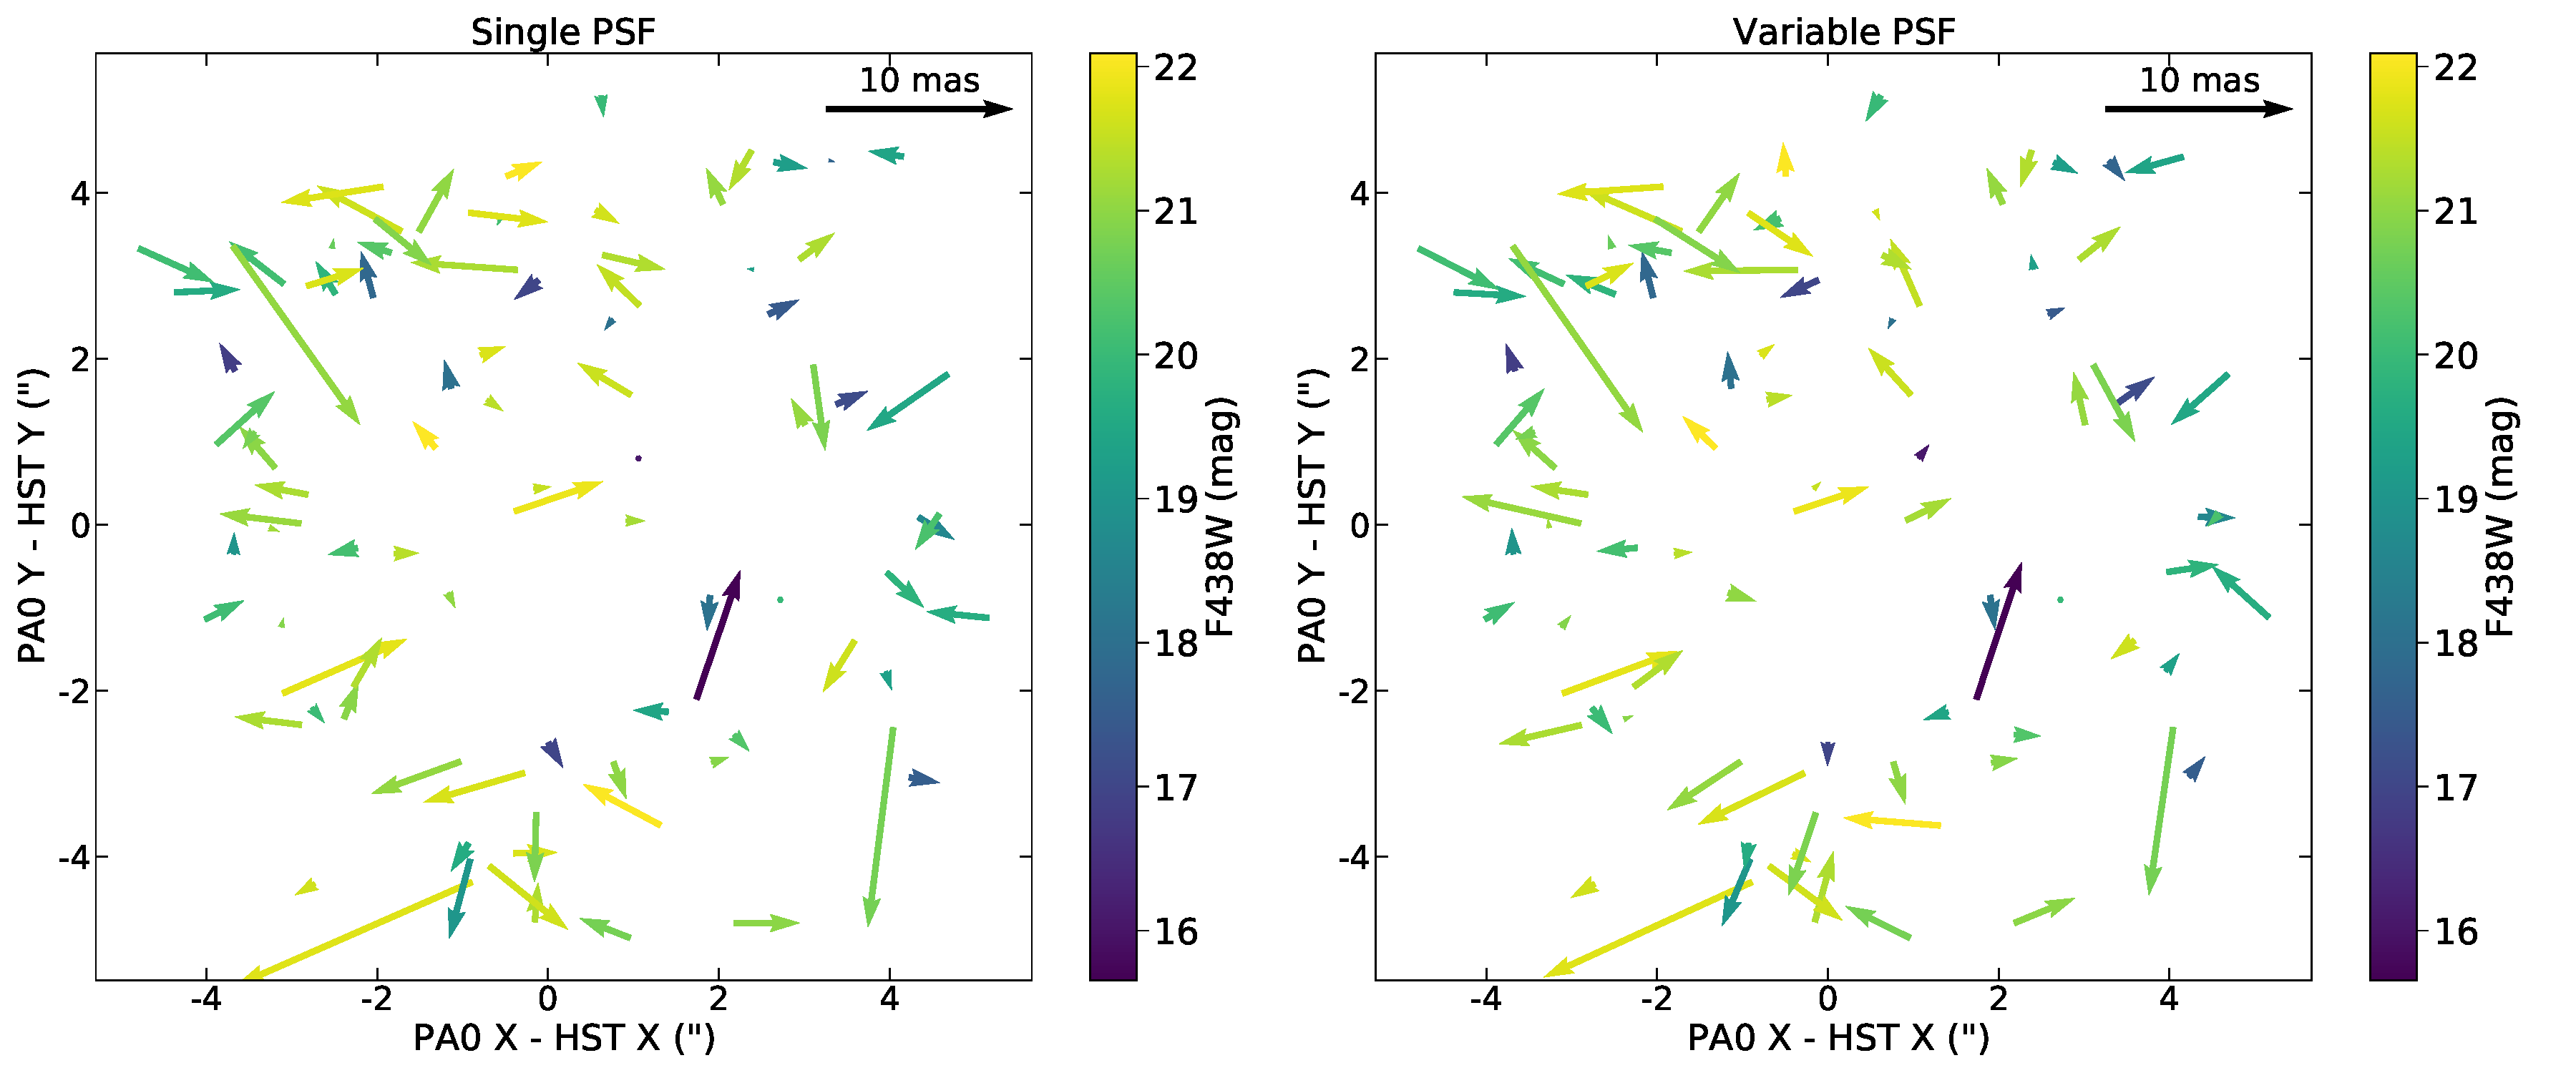
\includegraphics[width=0.95\textwidth]{Figures/m53-to-hst_both_matched_quivers.pdf}}\\
  \hspace{-1cm}
  \subfloat{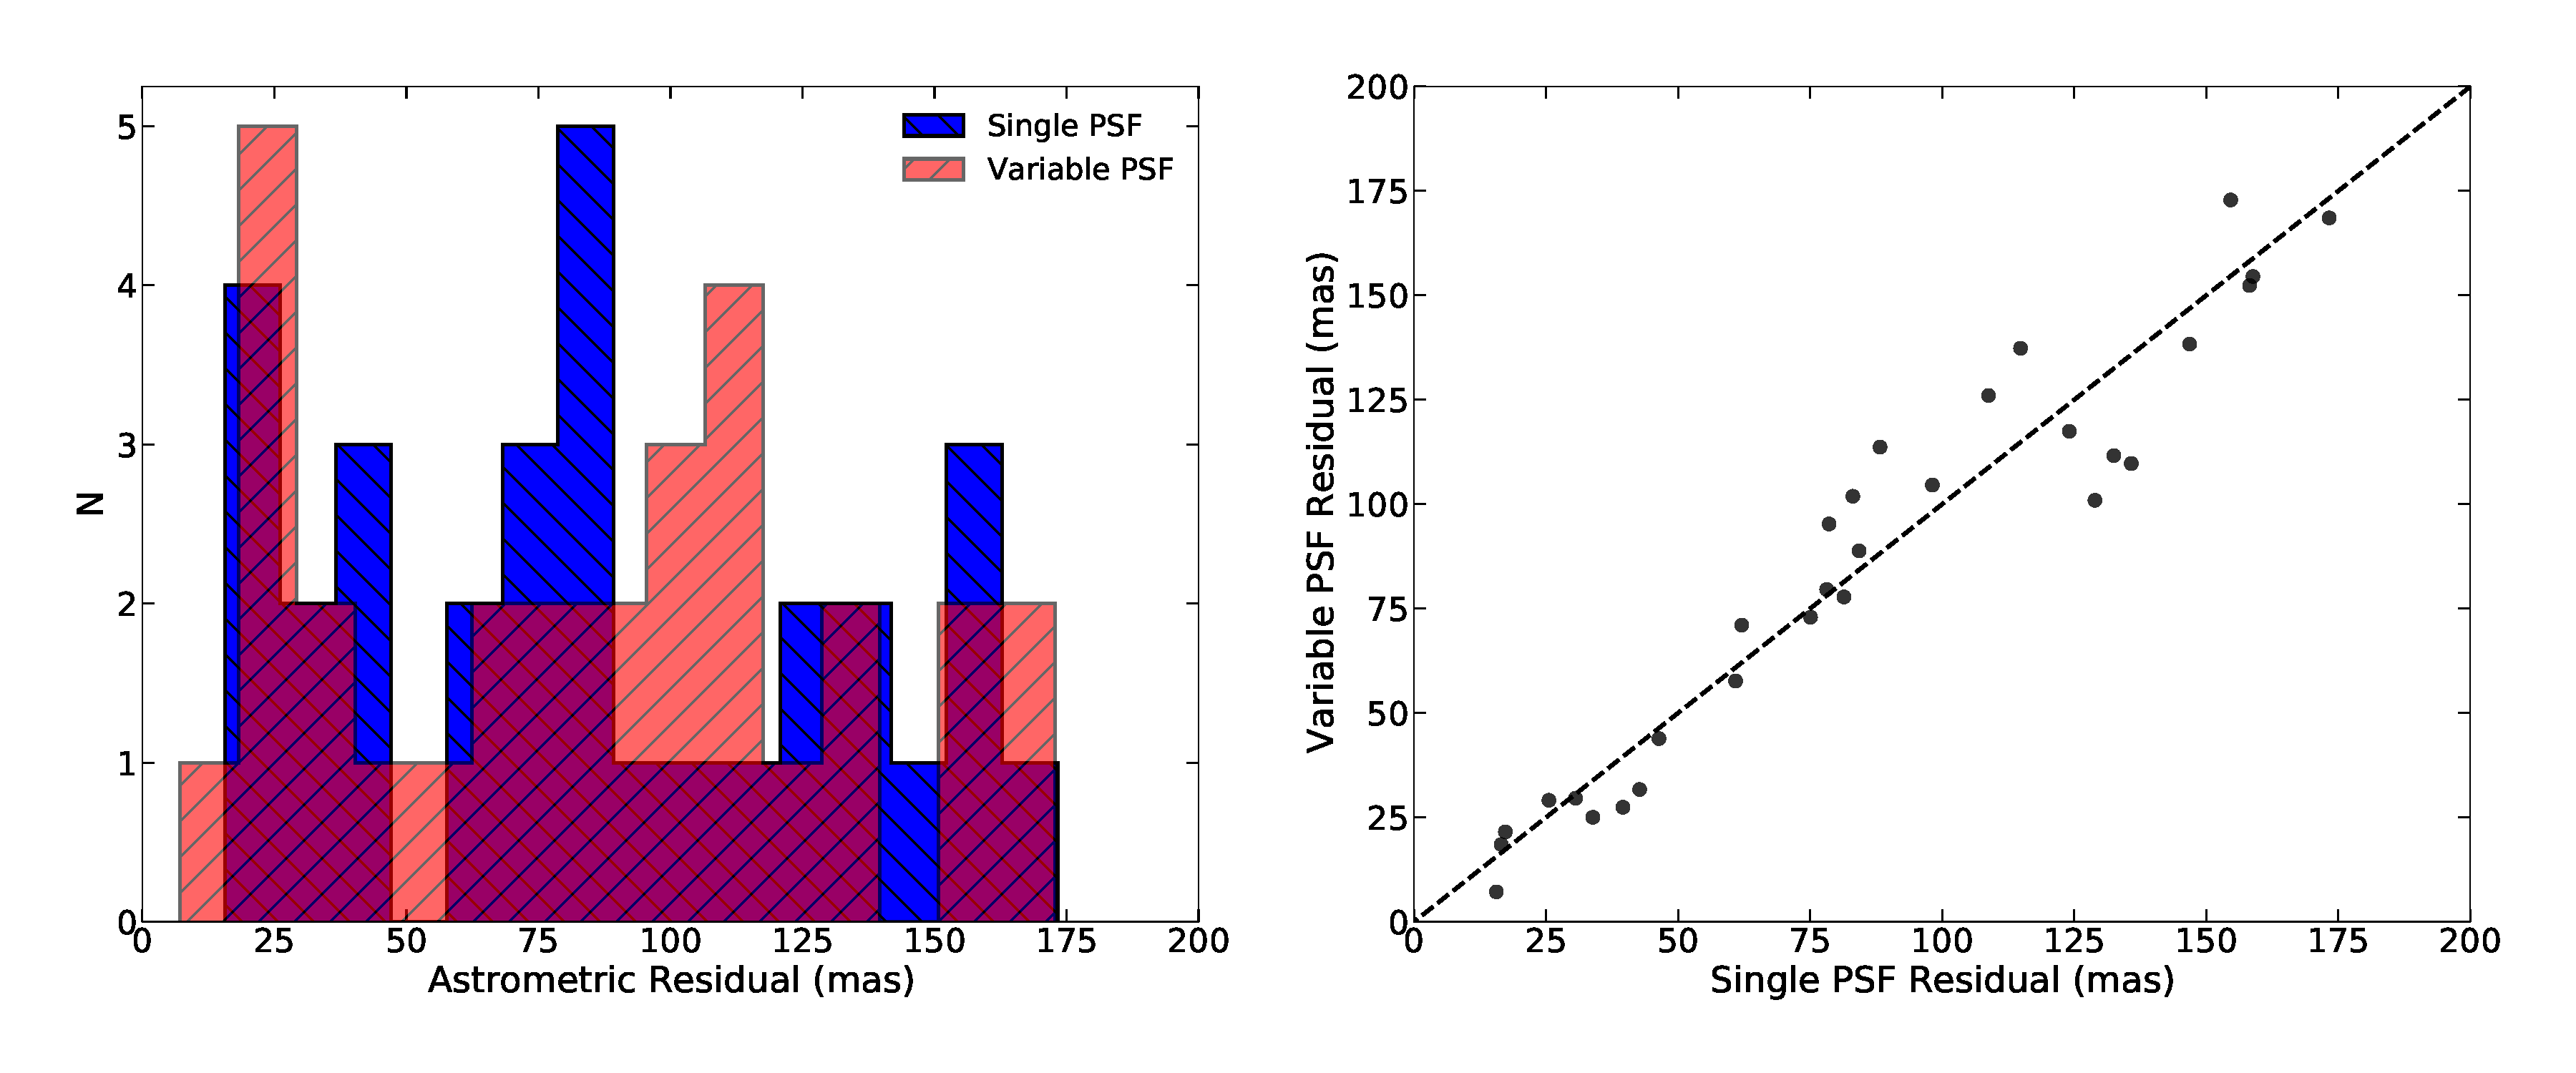
\includegraphics[width=0.95\textwidth]{Figures/m53-to-hst_histAndCorrelation.pdf}}
  \caption{Same as Figures \ref{fig:m53_PA_compare} and \ref{fig:m53_PA_compare_gaia}, but for stars matched and transformed to HST. The color bar is given in F814W (Vega) magnitude.} \label{fig:m53_PA_compare_hst}
\end{figure}

The M53 dataset includes six frames taken at a position angle of 0\degree (i.e. North up, East left), and six frames taken at a position angle of 90\degree (i.e. East up, South left). The PA $=0$ dataset consists of two frames taken at the central pointing, and four frames taken after a dither of $\Delta_x = -0.14", \Delta_y = 0.16"$. The PA $=90$ dataset consists of three frames taken at the central pointing, and three frames taken after a dither of $\Delta_x = +0.14", \Delta_y = -0.19"$. The total exposure time was 50 seconds per frame for both PAs. Figure \ref{fig:m53_image_grid} shows one frame taken at PA 0 and the accompanying grid of FWHM values from AIROPA variable-PSF mode, as well as a PA 90 frame and FWHM grid. The same TT guide star was used for both PAs, which has magnitude R ${\sim}$ 13.5 located 24 arcseconds to the Southwest.

AIROPA was run on all images at each PA using the same 10 PSF reference stars which are shown as data points colored by magnitude in the bottom panels of Figure \ref{fig:m53_image_grid}. Both the variable and single-PSF mode astrometric and photometric extractions were performed on each image. Additionally, stellar positions and magnitudes from the four central-pointing PA $=0$ frames were then averaged, and the averaged star list was transformed to the reference star list frame. We used the PA$=$90 star list as the reference list since the data is of higher quality than PA$=$0. The PA$=$0 dataset is measurably lower quality than the PA$=$90 dataset; $\overline{\textrm{SR}}_{0\degree} = 0.76^{*}\overline{\textrm{SR}}_{90\degree}$, $\overline{\textrm{FWHM}}_{0\degree}$ $= 1.14^{*}\overline{\textrm{FWHM}}_{90\degree}$.

%----------------FVU------------------------------------------------------------------------------------------------------------

\section{Fraction of Variance Unexplained} \label{sec:fvu}
An important metric that we use to determine the ``quality of the fit" for each PSF-mode inside AIROPA is the FVU. This metric is defined as the ratio between the variance of the residuals and the variance of the image itself, and is given by:

\begin{equation}
    FVU = \frac{\sigma^{2}_{\textrm{res}}}{\sigma^{2}_{\textrm{img}}}
\end{equation}

\noindent where $\sigma^{2}_{\textrm{res}}$ is the variance of the residual, and $\sigma^{2}_{\textrm{img}}$ is the variance of the image. According to \cite{Turri:inprep}, the FVU is only a reliable metric for brighter stars because they are minimally affected by noise, with the largest error contribution coming from systematics on the PSF. The lower panels of Figures \ref{fig:ob-m53-astrom} and \ref{fig:gc-astrom} show the single/variable FVU comparison for all six datasets, with further details given in section \ref{sec:fvu-astrom-results}. %This discrepancy was also discovered in \cite{Turri:inprep}, where they showed significant improvement to the FVU in simulated data, but effectively no improvement in on-sky comparisons. This implies that there are additional aberrations in the AO system that are not accounted for when moving from fiber source calibrations to on-sky science data.

%----------------Results------------------------------------------------------------------------------------------------------------

\section{Results} \label{sec:fvu-astrom-results}
Our analysis of six independent NIRC2 on-sky datasets show marginal or no improvement in astrometric residuals between the static PSF model and spatially variable PSF model within AIROPA. A comparison of the FVU metric between the two modes show similar results. This implies that the ability of AIROPA to reconstruct the PSF for a wide range on-sky data remains limited by unaccounted for aberrations in the telescope. We also show that the effect of varying atmospheric conditions, number and spatial location of selected PSF reference stars, and telescope PA do not have a significant effect on the performance of AIROPA in either of the modes.

\begin{figure}[!h]
 \makebox[\textwidth][c]{
 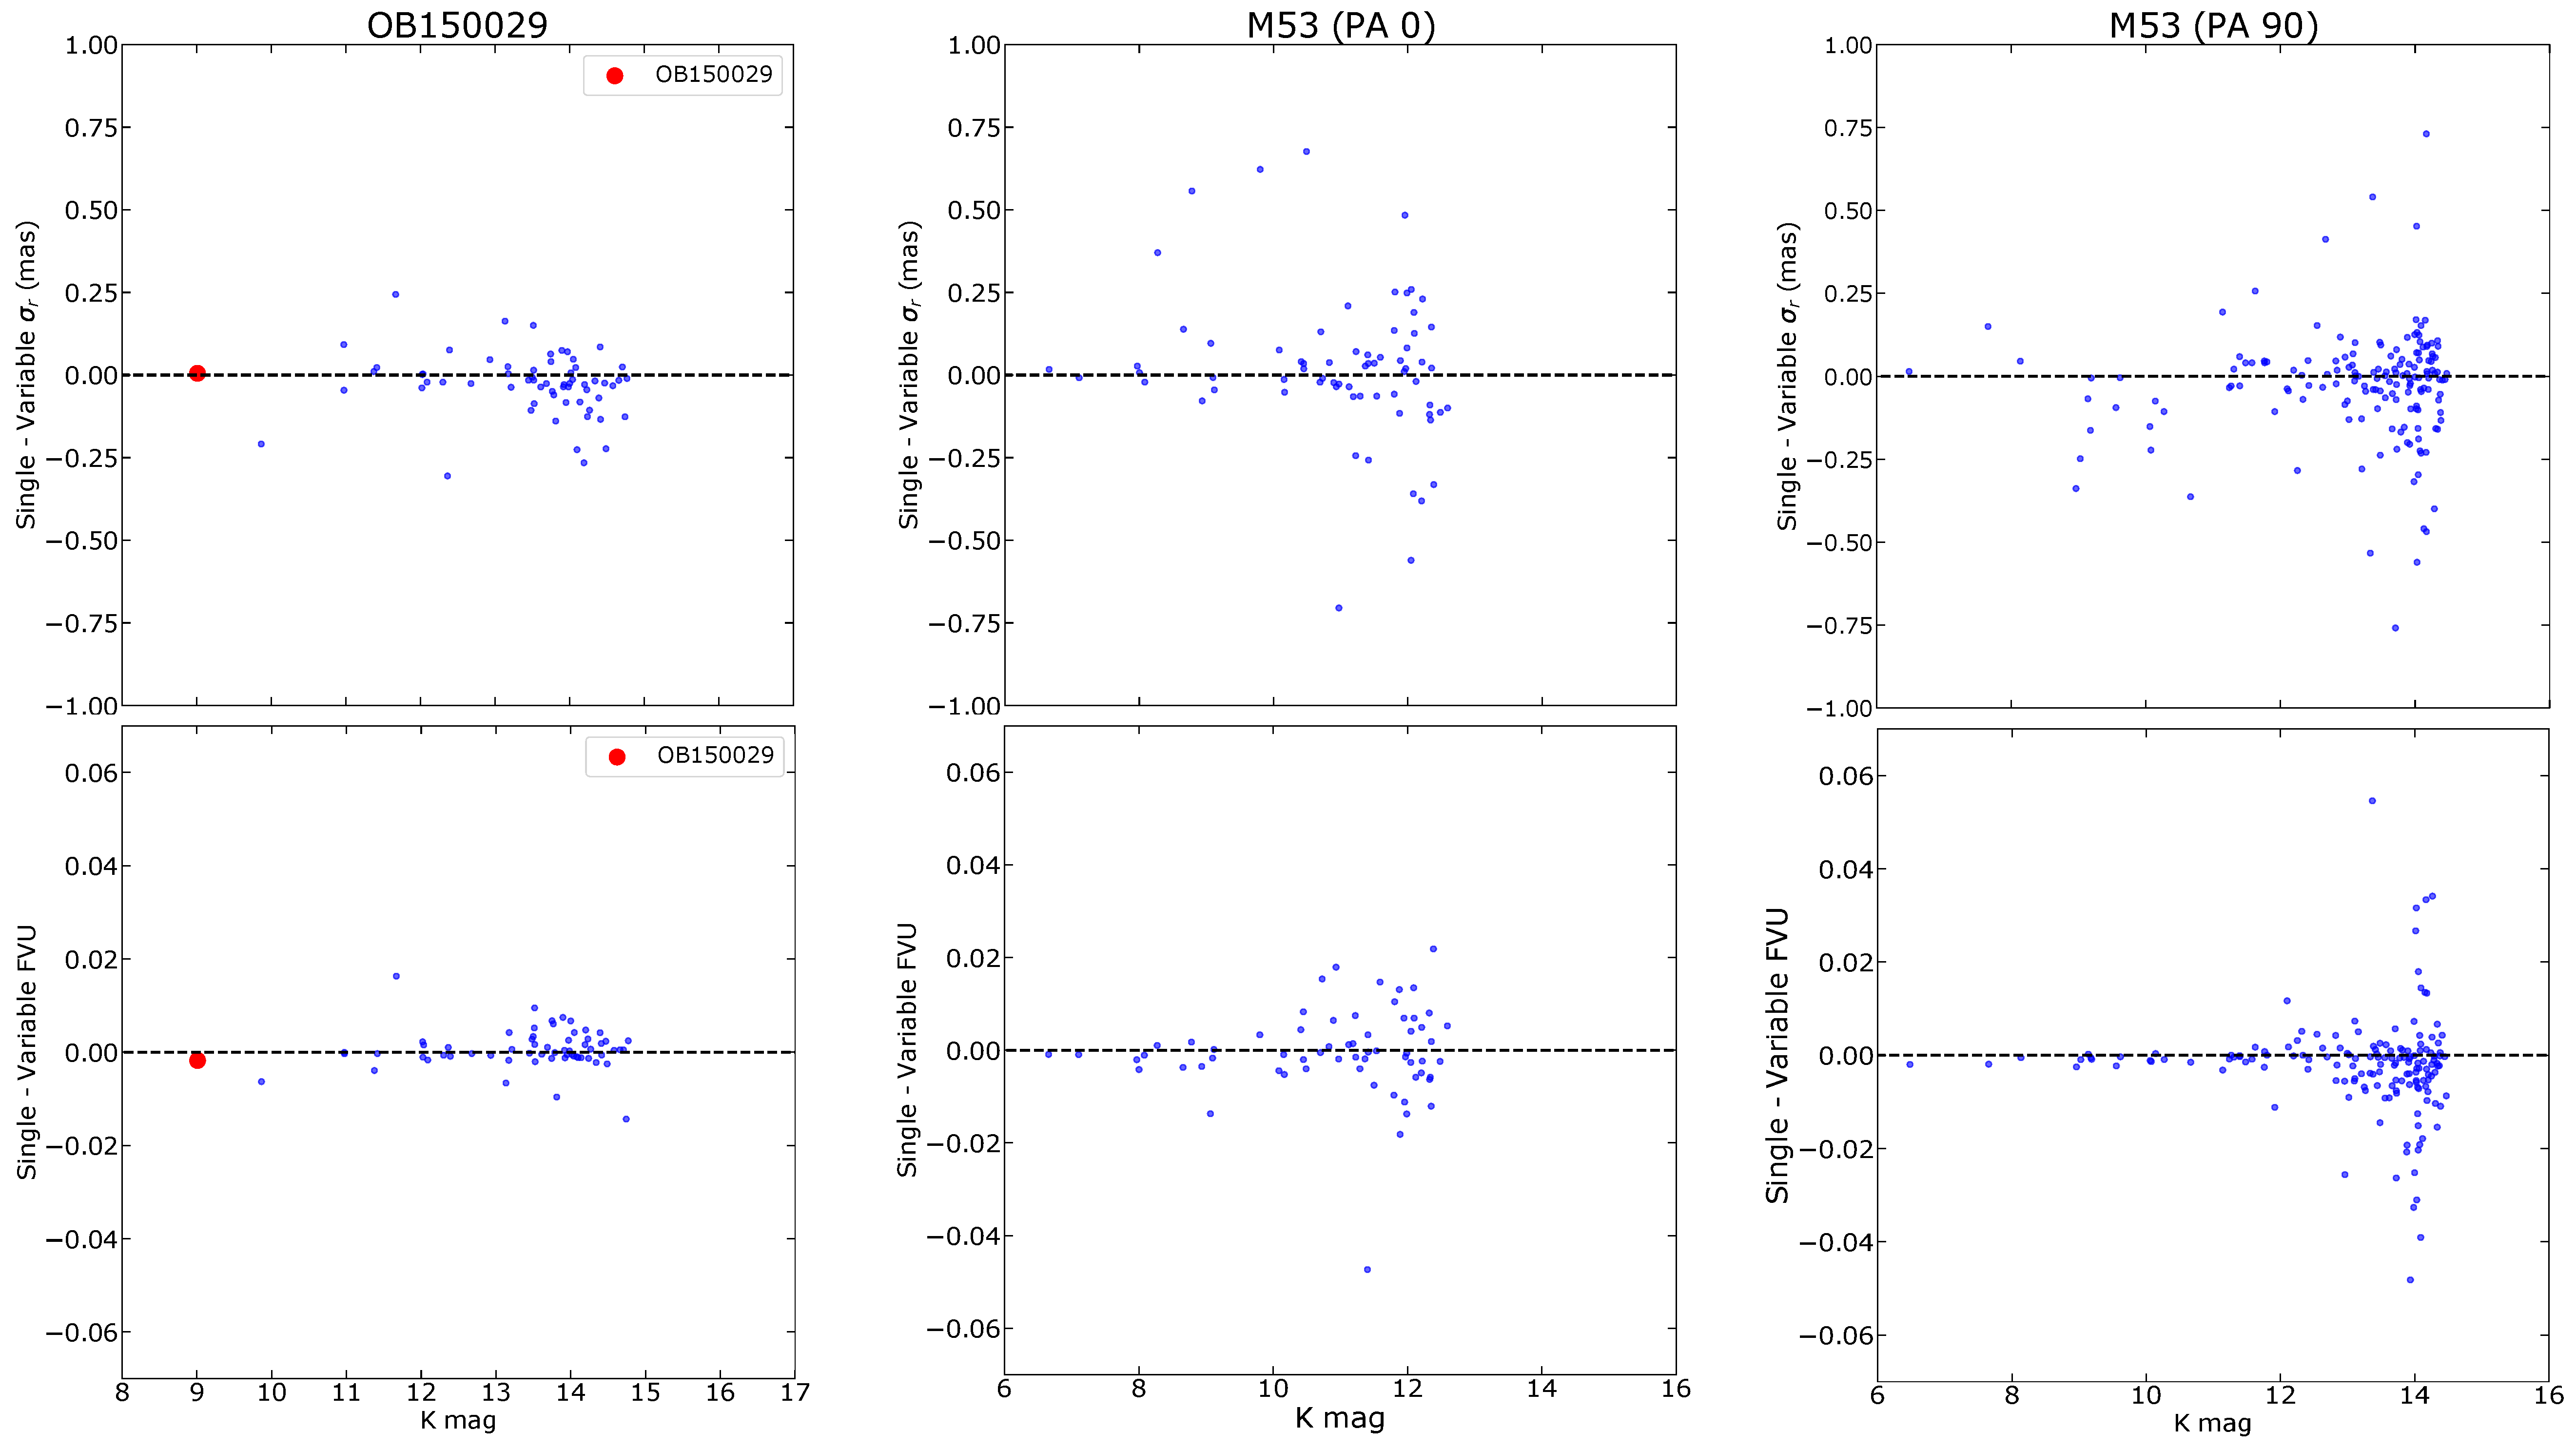
\includegraphics[width=1.1\textwidth]{Figures/ob-m53-astrometry-fvu.pdf}
 }
 \caption{\footnotesize Astrometric errors and correlations between single-PSF and variable-PSF modes for the datasets; OB150029 (\textit{left column}), M53 PA$=$0 (\textit{middle column}), and M53 PA$=$90 (\textit{right column}).} \label{fig:ob-m53-astrom}
\end{figure}

\indent For the microlensing target, OB150029, there is a marginal improvement of ${\sim}2\%$ in the astrometric precision in variable-PSF mode ($\sigma_{r}=0.226$ mas) over single-PSF mode ($\sigma_{r}=0.231$ mas). The upper-left panel of Figure \ref{fig:ob-m53-astrom} shows the astrometric residuals for all stars detected in both PSF modes, OB150029 is given as the red filled circle. Interestingly, the FVU metric for the target is worse (larger) with the variable-PSF ($3.90\times10^{-3}$) compared to the single-PSF ($2.14\times10^{-3}$)(lower-left panel of Figure \ref{fig:ob-m53-astrom}). 
%This is a ${\sim}43\%$ decrease in FVU for the single-PSF mode. A possible explanation for this is that target is the brightest star in the field and is used as a PSF reference star itself for the single mode to build the PSF model. Although the PSF reference stars are de-convolved and normalized to the same scale during the building of the PSF model inside AIROPA, there may still be some influence on the fitting and subtraction, particularly in the wings of the PSF. The case is clearly different for the spatially variable PSF model given the phase map and atmospheric profile information that is utilized in this mode.
The majority of the increased FVU comes from an over-subtracted region to the Northwest of the PSF core (right panel of Figure \ref{fig:ob150029-targ-res}).

\begin{figure}[!h]
 \makebox[\textwidth][c]{
 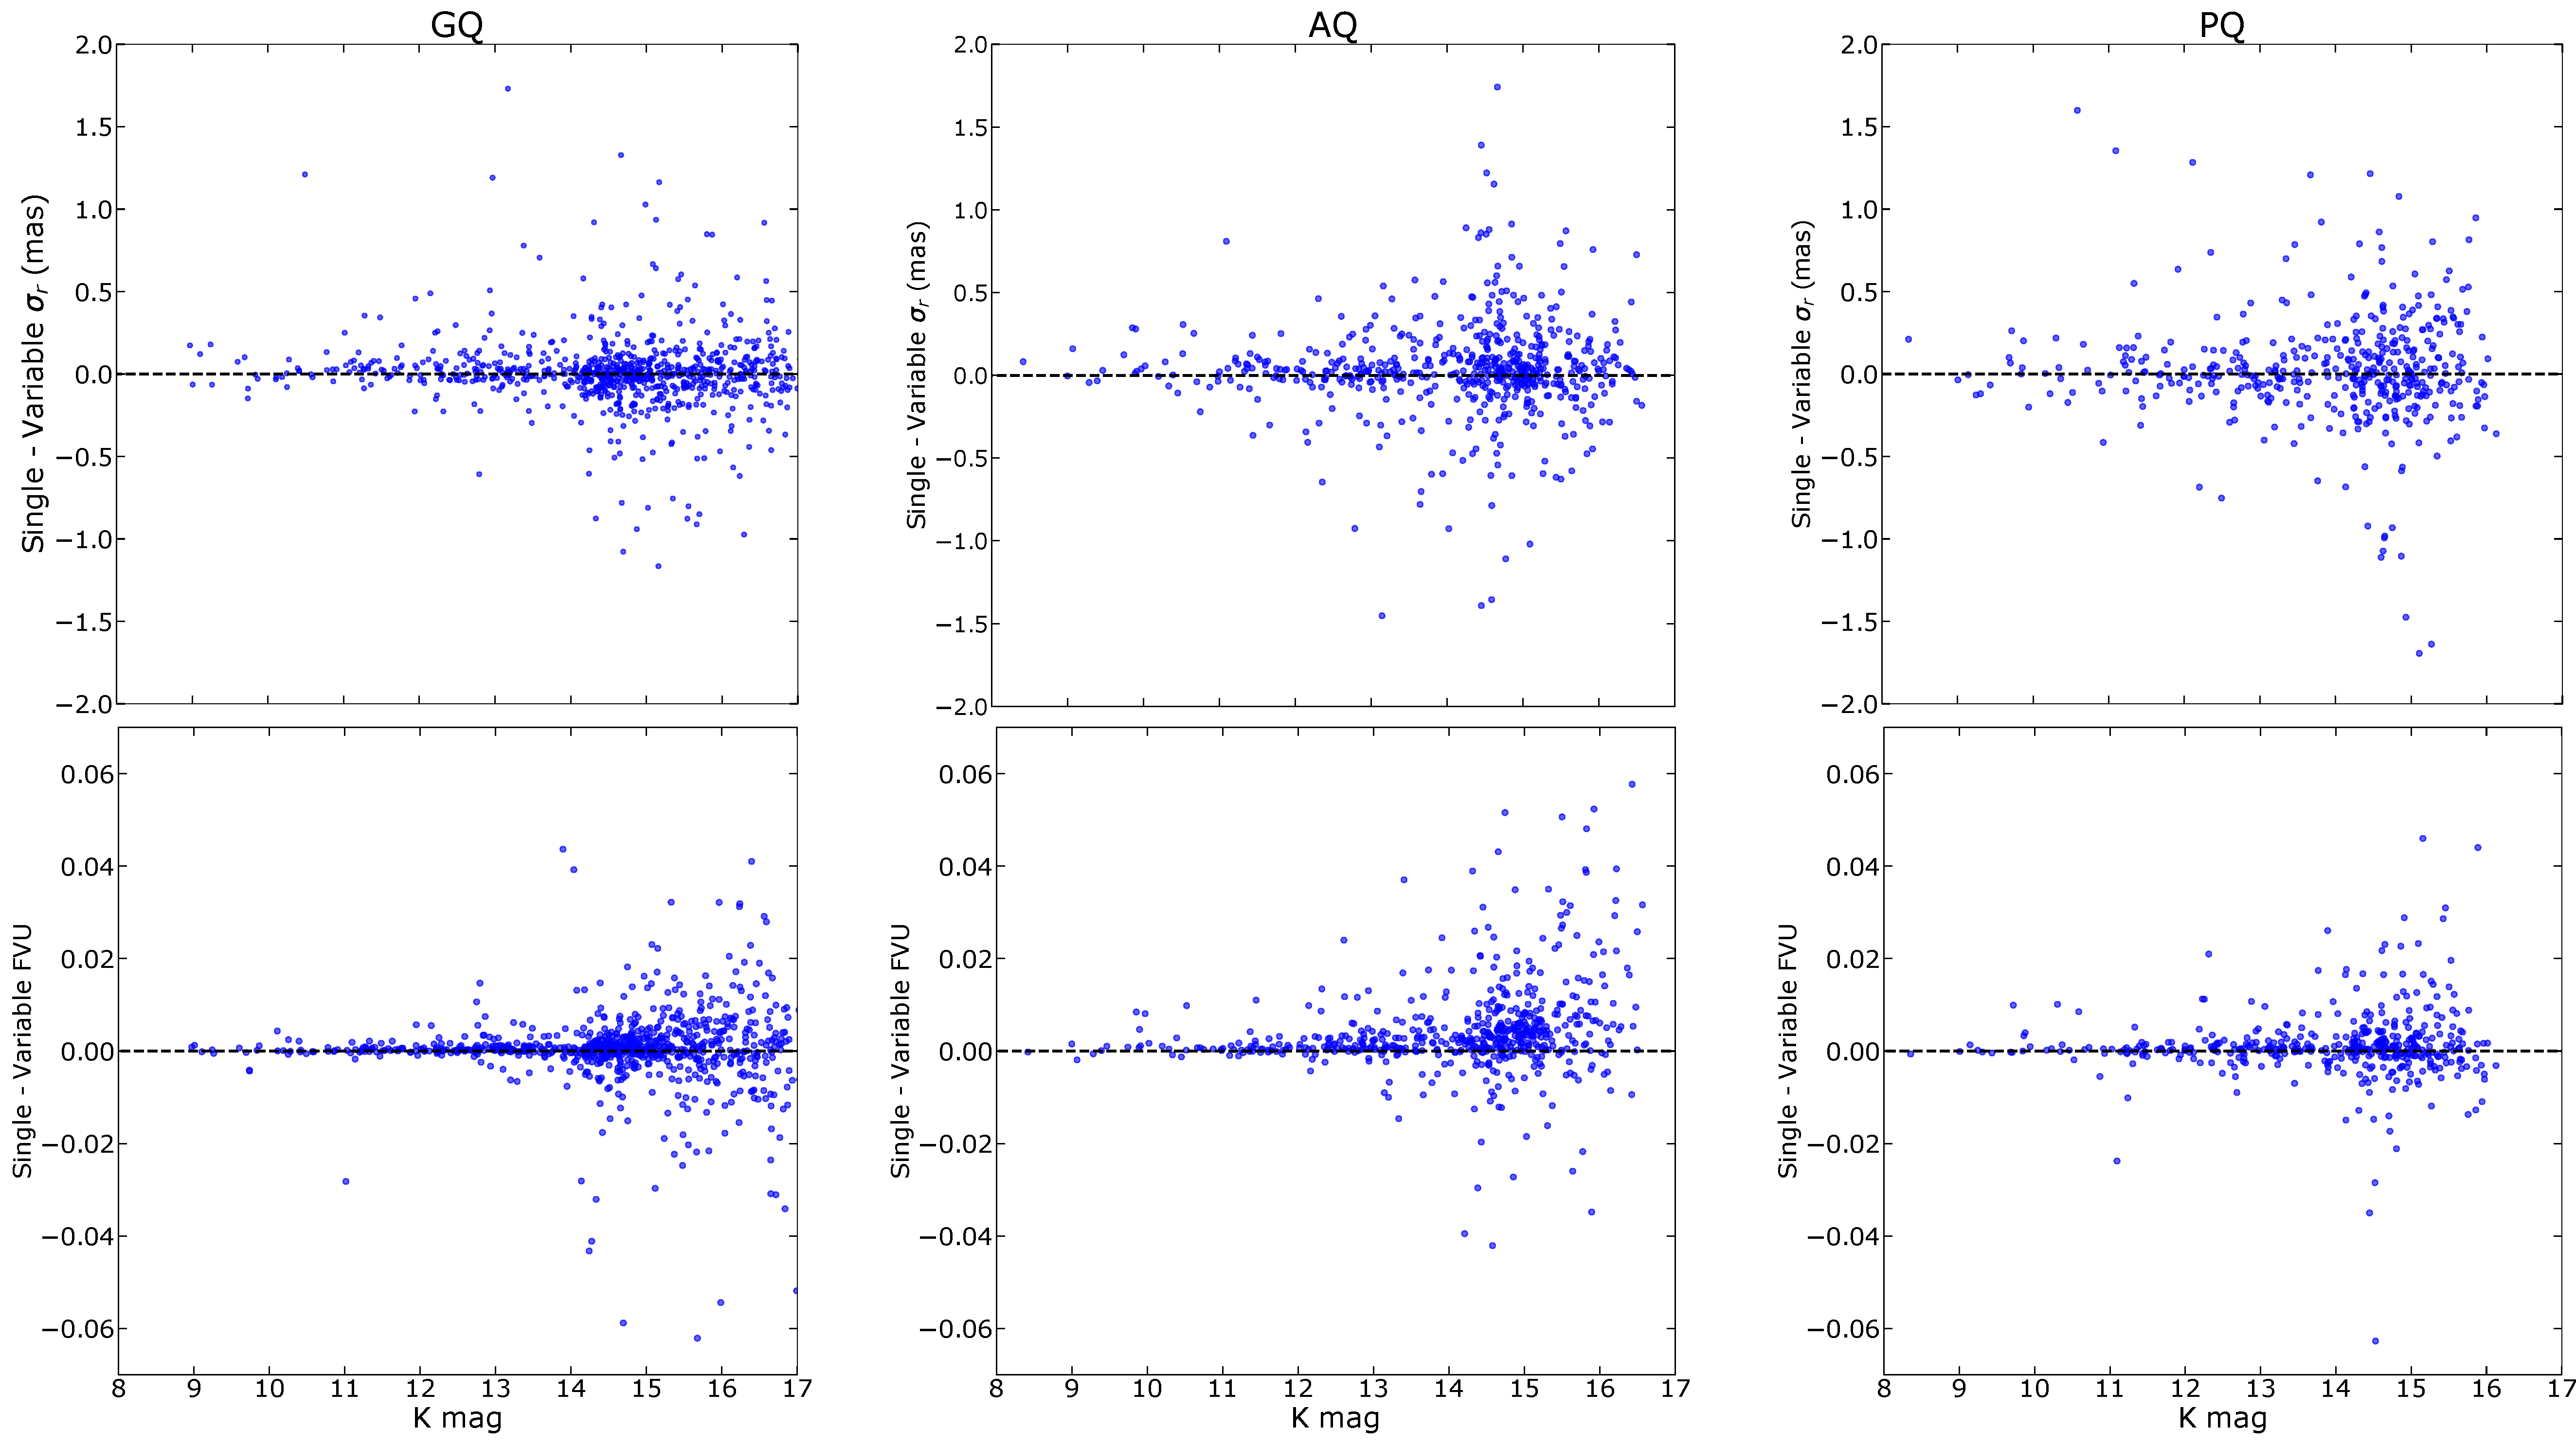
\includegraphics[width=1.1\textwidth]{Figures/gc-astrometry-fvu.pdf}
 }
 \caption{\footnotesize Same as Figure \ref{fig:ob-m53-astrom}, but for the GQ (\textit{left column}), AQ (\textit{middle column}), and PQ (\textit{right column}) datasets.} \label{fig:gc-astrom}
\end{figure}

%This likely effects the astrometric precision between the PA$=$0 $\rightarrow$ PA$=$90 transformation by $\sim$XX\%. 
For the M53 datasets, the astrometric precision is very similar between the two PSF modes for both PAs as can be seen in Figure \ref{fig:ob-m53-astrom}. Ignoring a few outliers, the FVU values between single and variable modes differ by ${\sim}$0.04 at most, with the largest spread at fainter magnitudes. The astrometric residuals after transforming the PA$=$0 star lists into the PA$=$90 reference frame have a dispersion of ${\sim}4$ mas, seen in the lower-right panel of Figure \ref{fig:m53_PA_compare}. The distribution of astrometric residuals for all cross-matched stars between the two PAs is also quite similar (lower-left panel of Figure \ref{fig:m53_PA_compare}), with a slightly smaller peak for variable-PSF ($\sigma_{r}\leq2$ mas) compared to single-PSF ($\sigma_{r}\geq2$ mas). 

The averaged starlists from both PA's were also matched and transformed to Gaia EDR3 \citep{brown:2021a}. There were a total of 32 matched stars between both PA's and Gaia, which can be seen in Figure \ref{fig:m53_PA_compare_gaia}. The quiver plots in the top panels of Figure \ref{fig:m53_PA_compare_gaia} look nearly identical because the astrometric differences between the two PSF modes is significantly smaller than the astrometric difference between the AIROPA and Gaia positions. The distribution of astrometric residuals for both PA's peaks at $\sigma_{r}\leq5$ mas, and the faintest stars have the largest residuals, as expected. The NIRC2 to Gaia matching show similar results to the PA$=$0 $\rightarrow$ PA$=$90 matching in terms of the astrometric residuals, albeit the Gaia residuals are larger as expected when transforming across different coordinate systems. Additional considerations need to be made when matching the two PA's to Gaia (i.e. astrometric fitting errors described in \cite{brown:2018a} and \cite{brown:2021a}). In particular the ``astrometric excess noise ($\epsilon$)" parameter is described simply as the excess uncertainty that must be added in quadrature to obtain a statistically acceptable astrometric solution. Further, the excess term $\epsilon$ is introduced in order to effectively reduce the statistical weight of observations that may be affected by things like instrument and attitude modeling errors. Of the ${\sim}$30 matched stars to Gaia, nearly all have $\epsilon < $ XXX, which we deem reliable/unreliable. More information on this error term is given in \cite{lindegren:2012a}. A final detail of this scheme is that the PSF-fitting and source extraction are not strictly centroid-conserving. This effect is particularly significant for off-axis stars that suffer from significant anisoplanatism.

Finally, the M53 starlists were transformed and matched to the HST reference frame using archival HST ACS data (as in \cite{service:2016a}). Figure \ref{fig:m53_PA_compare_hst} shows the astrometric residual quiver plots in the upper panels, and corresponding distribution of residuals. The astrometric residuals are much larger for the transformation to HST, and I'm not sure why.... I performed the transformation/matching similarly to the Gaia procedure. I also confirmed that the \textit{`order = 1'} flag performs only a simple rotation and translation. The Gaia output gives astrometric residuals in arcseconds (i.e. divide by 1000 for milliarcsecond), while the HST output gives astrometric residuals in pixels (i.e. multiple by 40 for milliarcsecond). Need to look at this result again I suppose.

%Significantly less stars were matched compared to the original study because, for the type of analysis presented in this work, we are limited to four un-dithered frames at PA$=0$ and three un-dithered frames at PA$=90$. While furthering the analysis of \cite{service:2016a} by implementing a variable-PSF-based distortion solution for both Keck-II/NIRC2 and Keck-I/OSIRIS would benefit from the current work, deriving this type of new distortion solution in the current work is beyond scope.

\indent For the much more crowded GC datasets, the average astrometric precision for the PQ stars with $m_{K} \leq 13$ is $\sigma_{{r}}{\sim}1.0$ mas for both single and variable-PSF modes. The average FVU metric is marginally better (smaller) for the variable-PSF ($11.7\times10^{-3}$) than for the single-PSF ($12.4\times10^{-3}$) for the bright sources in the frames. This improvement is much less than what has been measured on simulation tests in \cite{Turri:inprep}. Further, the results are much the same for both the AQ and GQ datasets. There is a marginal improvement in the average FVU for the GQ bright stars $m_{K} \leq 13$ with variable-PSF mode. The average FVU for the GQ variable-PSF mode is $5.34\times10^{-3}$, compared to the single-PSF mode average value of $5.58\times10^{-3}$. The differences in astrometric error and FVU for all of the GC datasets are given in Figure \ref{fig:gc-astrom}.

%\begin{figure}[!h]
 %\makebox[\textwidth][c]{
 %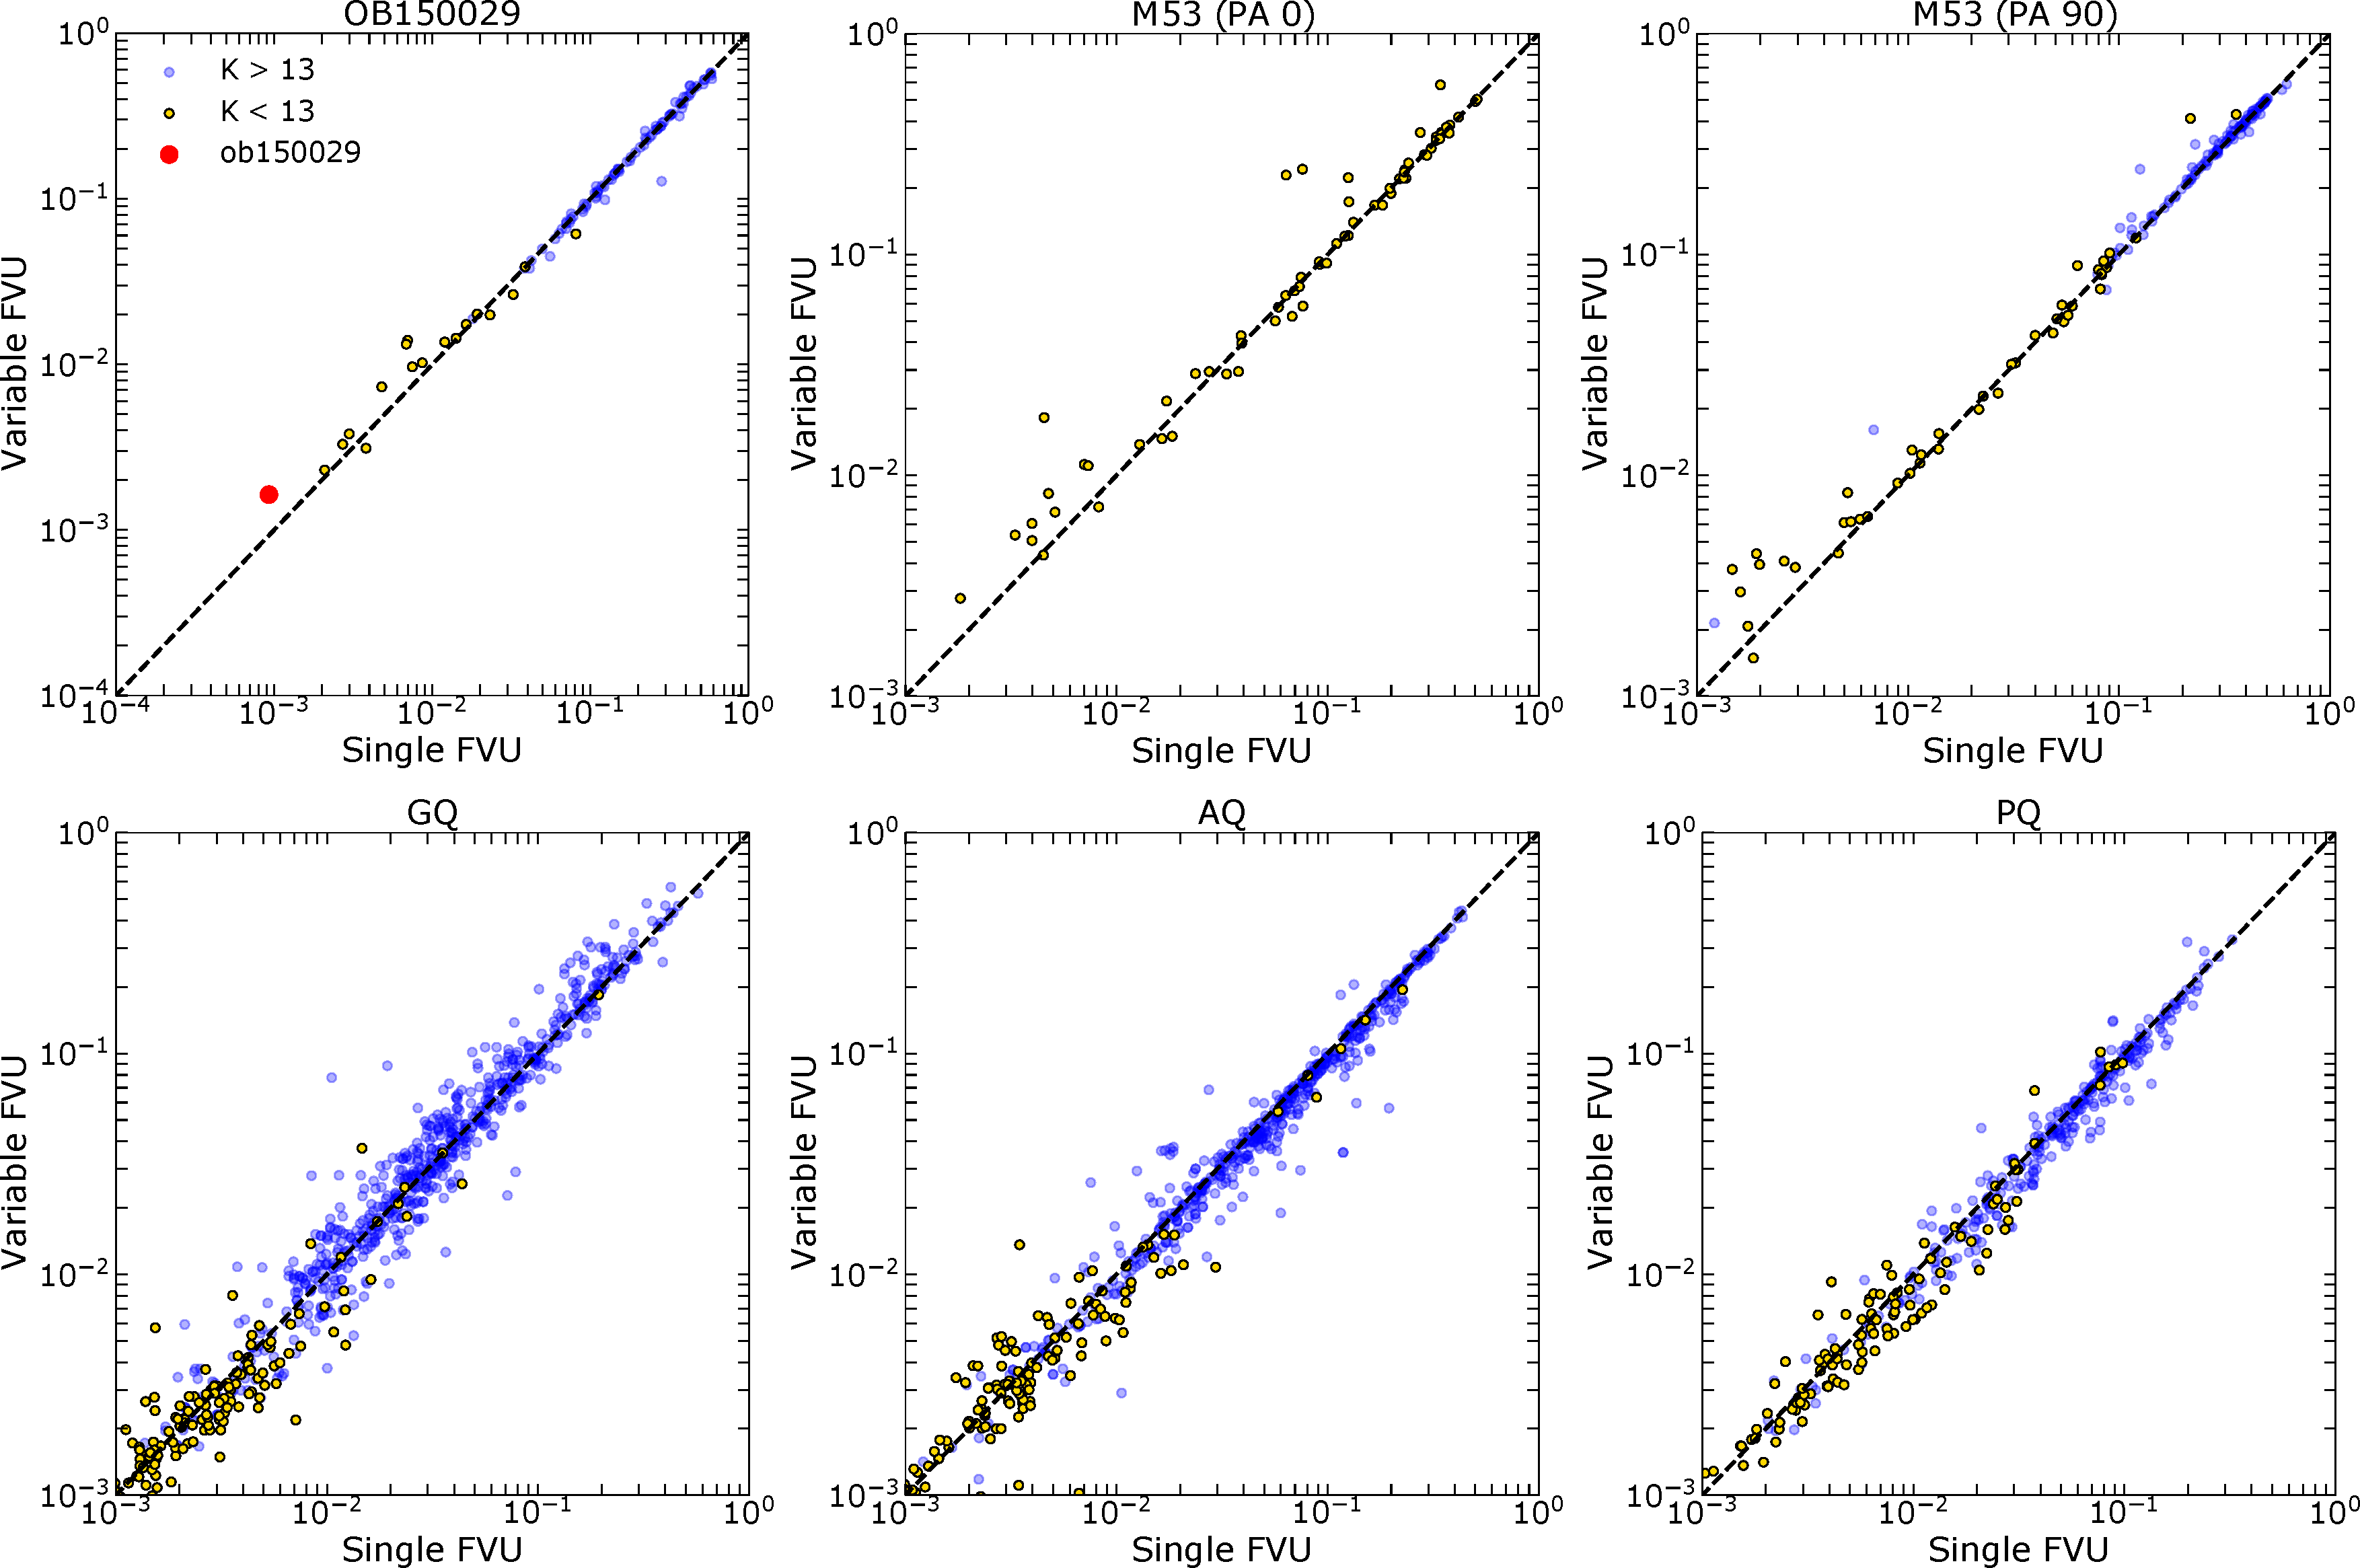
\includegraphics[width=1.0\textwidth]{Figures/fvu_grid.pdf}
 %}
 %\caption{\footnotesize \textit{Left Column}: M53 NIRC2 frame taken at PA = 0, with accompanying variable-PSF mode FWHM grid generated by AIROPA. \textit{Right Column}: Same as left, but for PA = 90.} \label{fig:fvu_grid}
%\end{figure}

%----------------Discussion and Conclusions------------------------------------------------------------------------------------------------------------

\section{Discussion and Conclusion} \label{sec:conclusion}

\indent We have analyzed several on-sky NIRC2 datasets with the the single PSF mode and spatially variable PSF mode in AIROPA. We find that the performance of AIROPA is reliable across different conditions including poor, average, and good quality seeing, crowded and/or sparse stellar fields, varying numbers and brightnesses of PSF reference stars, and in different telescope PA's.
\\
\indent Comparing the FVU metrics between PSF fitting modes across all datasets shows at best a ${\sim}5\%$ improvement in bright stars for the spatially varying PSF model over a static PSF model. This is significantly less than what has been shown in similar tests on simulated GC data \citep{Turri:inprep}. The biggest improvement in astrometric precision comes from the analysis of microlensing target OB150029. We measure an astrometric precision that is ${\sim}20\%$ smaller for the variable-PSF mode over the single-PSF mode. It is curious, however, that the FVU metric for this target does not follow this same improvement seen in the astrometry. For the M53 data, we find that the astrometric residuals are very similar when transforming a stack of PA $=$ 0 frames onto the PA $=$ 90 reference frame. When transforming the two PA's to the Gaia and HST reference, we find very similar results. This is because the astrometric differences between single-PSF and variable-PSF modes are much smaller than the residuals when matching either PSF modes astrometry to the absolute Gaia and/or HST astrometry.
\\
\indent We largely confirm the result of \cite{Turri:inprep} which shows no significant improvement in fitting residuals for the spatially variable PSF mode in AIROPA with on-sky data. It is hypothesized that there remains static or quasi-static instrumental aberrations that persist in the telescope and are not being fully characterized by afternoon phase diversity measurements. Future on-sky phase diversity measurements should help in identifying the source(s) of instrumental aberrations that are not currently accounted for in fiber phase diversity measurements. 

\acknowledgments

The data presented herein were obtained at the W. M. Keck Observatory, which is operated as a scientific partnership among the California Institute of Technology, the University of California and the National Aeronautics and Space Administration.
The Observatory was made possible by the generous financial support of the W. M. Keck Foundation.
The authors wish to recognize and acknowledge the very significant cultural role and reverence that the summit of Maunakea has always had within the indigenous Hawaiian community.
We are most fortunate to have the opportunity to conduct observations from this mountain.
\\
\indent SKT acknowledges support from the NSF through grant AST-1836016. We acknowledge support from the W. M. Keck Foundation, the Heising-Simons Foundation, the Gordon and Betty Moore Foundation, and the NSF (AST-1412615, AST-1518273). We thank the staff of Keck Observatory for their help with obtaining calibration data and overall support for our program.

%\begin{figure*}
%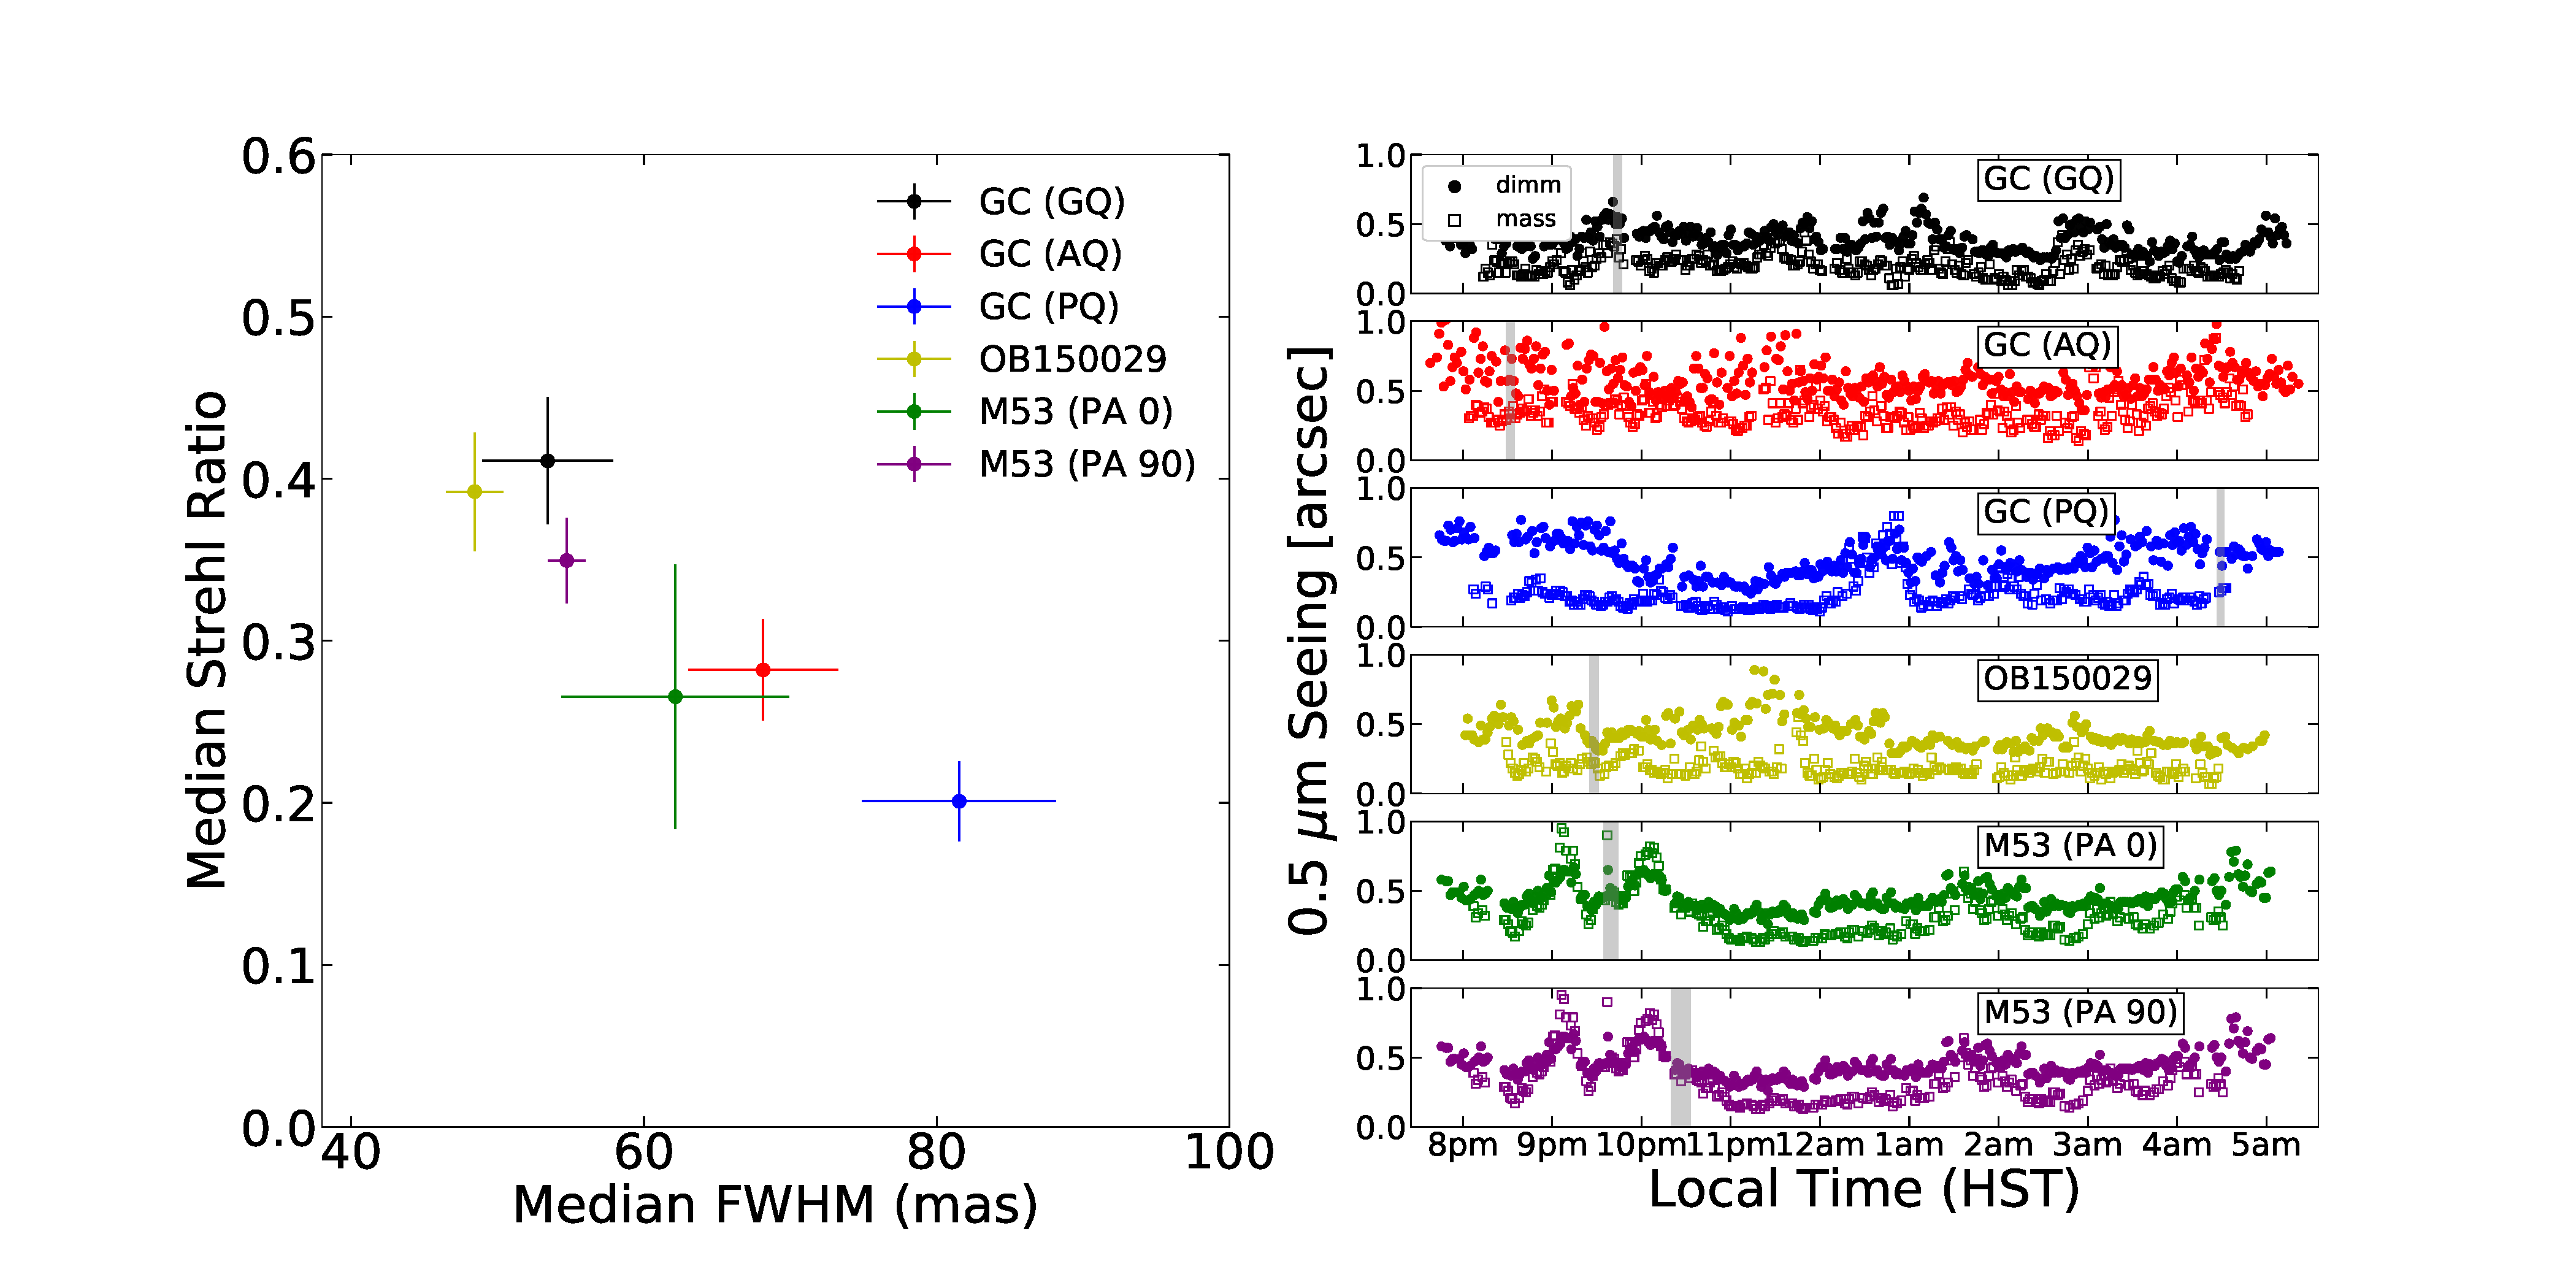
\includegraphics[width=\textwidth]{Figures/metrics_dimmmass.pdf}
%\caption{\footnotesize \textit{Left}: Strehl ratio and FWHM median and standard deviation for all datasets analyzed in this work. \textit{Right}: 0.5$\mu m$ DIMM/MASS seeing profiles for each dataset, respectively. Grey shaded region represents time of observation for each set. Six cleaned frames were analyzed for the GC and OB150029, and eight frames were analyzed for M53 (both PA's).} \label{fig:strehl_fwhm_dimmmass}
%\end{figure*}

\clearpage
% References
\bibliography{refs} % bibliography data in report.bib
\bibliographystyle{spiebib} % makes bibtex use spiebib.bst

%Exclude Appendix
%\appendix
%----------------PSF Clipping------------------------------------------------------------------------------------------------------------
%\section{PSF Clipping} \label{appendix:A}
%We have found that the PSF clipping process in AIROPA varies sensitively with the combined (instrumental + atmospheric) OTF, which for the latter is constructed using the closest available DIMM/MASS data to the observation. This is somewhat expected as the atmospheric contribution to the OTF relies on an accurate accounting of the total integrated $C_n^2$ profile across six turbulence layers in the atmosphere (0.5km, 1km, 2km, 4km, 8km, and 16km altitudes). The theoretical estimation of the total isoplanatic seeing is given as:

%\begin{equation}
%    \sigma_{\textrm{iso}} = 
%\end{equation}

%\noindent where ...

%We compared the atmospheric profiles for two different ``poor quality" datasets (hereafter PQ1 and PQ2). Each of the six PQ1 frames analyzed with AIROPA shows varying levels of PSF clipping near the core of the reconstructed PSF. Although the six frames from PQ2 are of similar Strehl Ratio and FWHM as PQ1, they do not show any signs of excessive PSF clipping from the algorithm.

%----------------PSF Smoothing------------------------------------------------------------------------------------------------------------
%\section{PSF Smoothing} \label{appendix:B}
%AIROPA has the capability to smooth the halo of the PSF. This function is useful to smooth out any background noise contribution that remains in the final PSF model. In order to validate the efficiency of this algorithm, we test the PSF smoothing function on one frame from the PQ dataset and one frame from an unrelated low-quality GC dataset that shows persistent background noise in the PSF halo. 

%Specifically, the PSF smoothing algorithm applies a variable box size median smoothing technique to the halo of the modeled PSF, where the radius that the smoothing function begins is user-defined. The smoothing calculation itself can be expressed as:

%\begin{equation}
%    \Phi_{i,j} = \sum_{i,j}(\mathrm{AW}_{i,j} + \mathrm{RW}_{i,j})
%\end{equation}

%where $\Phi_{i,j}$ is the two-dimensional smoothed PSF model, AW and RW are the azimuthal and radial width's for filtering. 

%\begin{figure}[!h]
% \makebox[\textwidth][c]{
% 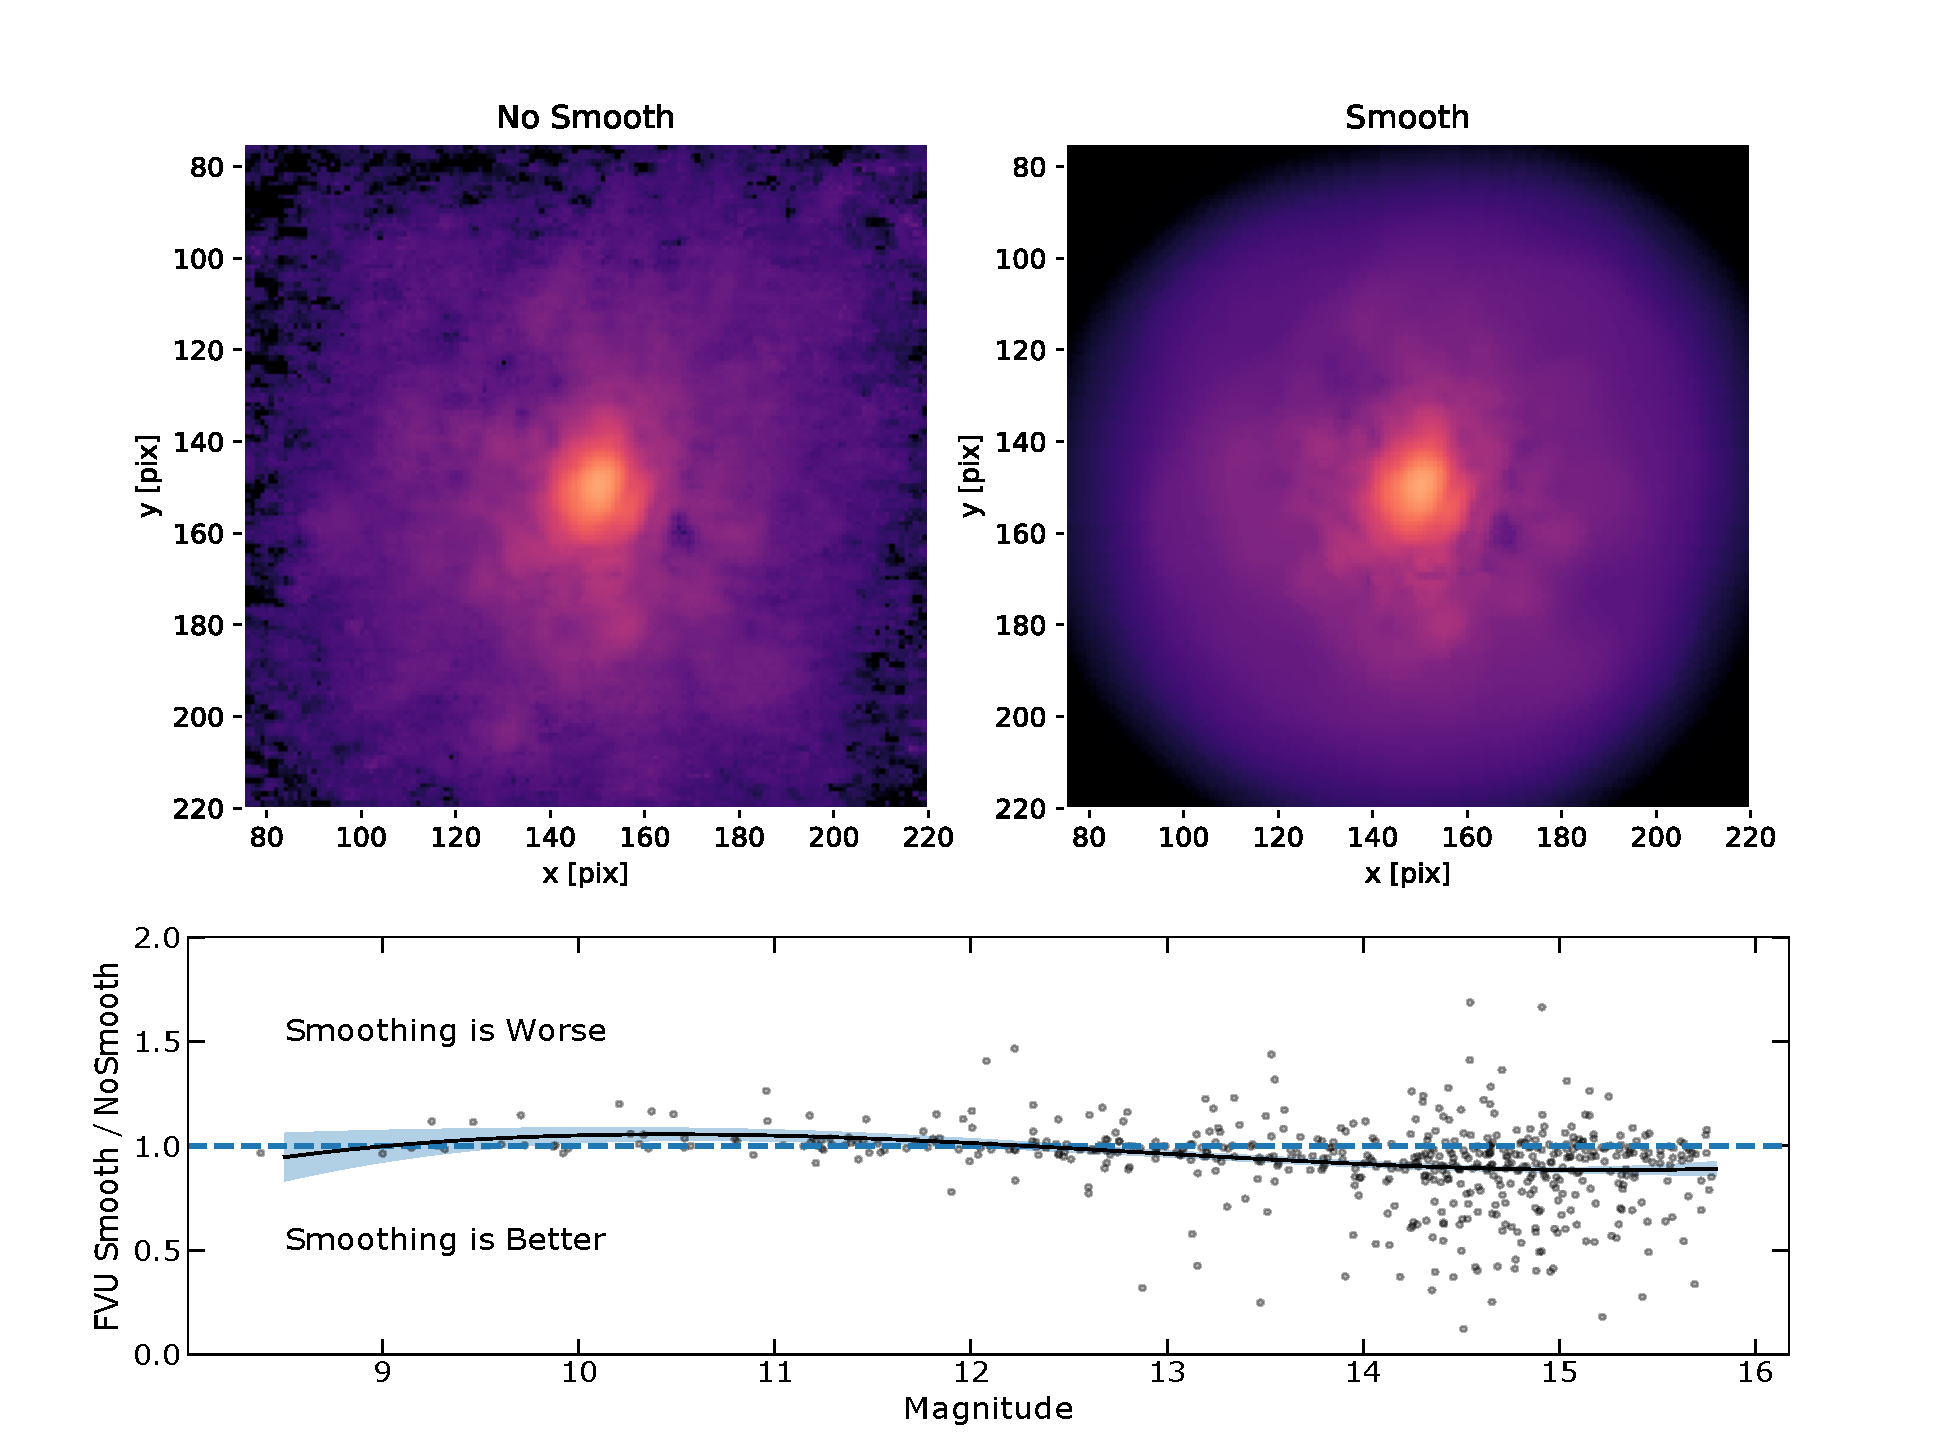
\includegraphics[width=0.8\textwidth]{Figures/fvu_smoothing.pdf}
% }
 %\caption{\footnotesize \textit{Top panel}: The extracted on-axis PSF from AIROPA variable-PSF mode showing the non-halo-smoothed PSF (left) and halo-smoothed PSF (right). \textit{Bottom panel}: The FVU ratio between smoothed and non-smoothed halo. Halo smoothing leads to better FVU values for fainter sources, and worse FVU values for bright sources. The solid black line shows a third-order polynomial fit, with blue shaded region representing 1$\sigma$ spread about the mean-fit.} \label{fig:fvu-smoothing}
%\end{figure}

\end{document} 
